\documentclass[12pt, a4paper, oneside, openright, titlepage]{book}
\usepackage[utf8]{inputenc}
\raggedbottom
\usepackage{import}


%%%%%%%%%%%%%%%%% Book Formatting Comments:

%%%%%%%%%%%%%%%%%%%%%%%%%%%%%%%%%%%%% for Part

%%%%%%%%%%%%%%%%%%%%%% for chapter

%%%%%%%%%%%%%%%%%%%% for section








%%%%%% PACKAGES %%%%%%%
\usepackage{hyperref}
\hypersetup{
    colorlinks,
    citecolor=black,
    filecolor=black,
    linkcolor=black,
    urlcolor=black
}
\usepackage{amsmath} % Math display options
\usepackage{amssymb} % Math symbols
\usepackage{amsfonts} % Math fonts
\usepackage{amsthm}
\usepackage{mathtools} % General math tools
\usepackage{array} % Allows you to write arrays
\usepackage{empheq} % For boxing equations
\usepackage{mathabx}
\usepackage{mathrsfs}
\usepackage{nameref}

\usepackage{soul}
\usepackage[normalem]{ulem}

\usepackage{txfonts}
\usepackage{cancel}
\usepackage[toc, page]{appendix}
\usepackage{titletoc,tocloft}
\setlength{\cftchapindent}{1em}
\setlength{\cftsecindent}{2em}
\setlength{\cftsubsecindent}{3em}
\setlength{\cftsubsubsecindent}{4em}
\usepackage{titlesec}

\titleformat{\section}
  {\normalfont\fontsize{25}{15}\bfseries}{\thesection}{1em}{}
\titleformat{\section}
  {\normalfont\fontsize{20}{15}\bfseries}{\thesubsection}{1em}{}
\setcounter{secnumdepth}{1}  
  
  

\newcommand\numberthis{\refstepcounter{equation}\tag{\theequation}} % For equation labelling
\usepackage[framemethod=tikz]{mdframed}

\usepackage{tikz} % For drawing commutative diagrams
\usetikzlibrary{cd}
\usetikzlibrary{calc}
\tikzset{every picture/.style={line width=0.75pt}} %set default line width to 0.75p

\usepackage{datetime}
\usepackage[margin=1in]{geometry}
\setlength{\parskip}{1em}
\usepackage{graphicx}
\usepackage{float}
\usepackage{fancyhdr}
\setlength{\headheight}{15pt} 
\pagestyle{fancy}
\lhead[\leftmark]{}
\rhead[]{\leftmark}

\usepackage{enumitem}

\usepackage{url}
\allowdisplaybreaks

%%%%%% ENVIRONMENTS %%%
\definecolor{purp}{rgb}{0.29, 0, 0.51}
\definecolor{bloo}{rgb}{0, 0.13, 0.80}



%%\newtheoremstyle{note}% hnamei
%{3pt}% hSpace above
%{3pt}% hSpace belowi
%{}% hBody fonti
%{}% hIndent amounti
%{\itshape}% hTheorem head fonti
%{:}% hPunctuation after theorem headi
%{.5em}% hSpace after theorem headi
%{}% hTheorem head spec (can be left empty, meaning ‘normal’)i


%%%%%%%%%%%%% THEOREM STYLES

\newtheoremstyle{BigTheorem}
{20pt}
{20pt}
{\slshape}
{}
{\Large\color{purp}\bfseries}
{.}
{\newline}
{\thmname{#1}\thmnumber{ #2}\thmnote{ (#3)}}



\newtheoremstyle{TheoremClassic}
{15pt}
{15pt}
{\slshape}
{}
{\bfseries}
{.}
{.5em}
{}

\newtheoremstyle{Definitions}
{15pt}
{15pt}
{\slshape}
{}
{\bfseries}
{.}
{.5em}
{\thmname{#1}\thmnumber{ #2}\thmnote{ (#3)}}


\newtheoremstyle{Remarks}
{10pt}
{10pt}
{\upshape}
{}
{\bfseries}
{.}
{.5em}
{}

\newtheoremstyle{Examples}
{10pt}
{10pt}
{\upshape}
{}
{\bfseries}
{.}
{.5em}
{}


%%%%%%%%%%%%% THEOREM DEFINITIONS

\theoremstyle{BigTheorem}
\newtheorem{namthm}{Theorem}
\newtheorem{conj}[namthm]{Conjecture}

\theoremstyle{TheoremClassic}
\newtheorem{thm}{Theorem}[section]
\newtheorem*{thm*}{Theorem}
\newtheorem{lem}[thm]{Lemma}
\newtheorem{cor}[thm]{Corollary}
\newtheorem{prop}[thm]{Proposition}
\newtheorem{claim}[thm]{Claim}


\theoremstyle{Definitions}
\newtheorem{defn}{Definition}[section]
\newtheorem{axi}[defn]{Axiom}
\newtheorem{cust}[defn]{}
\newtheorem{cons}[defn]{Construction}
\newtheorem{props}[defn]{Properties}
\newtheorem{proc}[defn]{Process}
\newtheorem*{law}{Law}


\theoremstyle{Examples}
\newtheorem{eg}{Example}[section]
\newtheorem{noneg}[eg]{Non-Example}
\newtheorem{xca}[eg]{Exercise}


\theoremstyle{Remarks}
\newtheorem{rmk}{Remark}[section]
\newtheorem{qst}[rmk]{Question}
\newtheorem*{ans}{Answer}
\newtheorem{obs}[rmk]{Observation}
\newtheorem{rec}[rmk]{Recall}
\newtheorem{summ}[rmk]{Summary}
\newtheorem{nota}[rmk]{Notation}
\newtheorem{note}[rmk]{Note}



\renewcommand{\qedsymbol}{$\blacksquare$}


\numberwithin{equation}{section}

\newenvironment{qest}{
    \begin{center}
        \em
    }
    {
    \end{center}
    }

%%%%%% MACROS %%%%%%%%%
%% New Commands
\newcommand{\ip}[1]{\langle#1\rangle} %%% Inner product
\newcommand{\abs}[1]{\lvert#1\rvert} %%% Modulus
\newcommand\diag{\operatorname{diag}} %%% diag matrix
\newcommand\tr{\mbox{tr}\.} %%% trace
\newcommand\C{\mathbb C} %%% Complex numbers
\newcommand\R{\mathbb R} %%% Real numbers
\newcommand\Z{\mathbb Z} %%% Integers
\newcommand\Q{\mathbb Q} %%% Rationals
\newcommand\N{\mathbb N} %%% Naturals
\newcommand\F{\mathbb F} %%% An arbitrary field
\newcommand\ste{\operatorname{St}} %%% Steinberg Representation
\newcommand\GL{\mathbf{GL}} %%% General Linear group
\newcommand\SL{\mathbf{SL}} %%% Special linear group
\newcommand\gl{\mathfrak{gl}} %%% General linear algebra
\newcommand\G{\mathbf{G}} %%% connected reductive group
\newcommand\g{\mathfrak{g}} %%% Lie algebra of G
\newcommand\Hbf{\mathbf{H}} %%% Theta fixed points of G
\newcommand\X{\mathbf{X}} %%% Symmetric space X
\newcommand{\catname}[1]{\normalfont\textbf{#1}}
\newcommand{\Set}{\catname{Set}} %%% Category set
\newcommand{\Grp}{\catname{Grp}} %%% Category group
\newcommand{\Rmod}{\catname{R-Mod}} %%% Category r-modules
\newcommand{\Mon}{\catname{Mon}} %%% Category monoid
\newcommand{\Ring}{\catname{Ring}} %%% Category ring
\newcommand{\Topp}{\catname{Top}} %%% Category Topological spaces
\newcommand{\Vect}{\catname{Vect}_{k}} %%% category vector spaces'
\newcommand\Hom{\mathbf{Hom}} %%% Arrows

\newcommand{\map}[2]{\begin{array}{c} #1 \\ #2 \end{array}}

\newcommand{\Emph}[1]{\textbf{\ul{\emph{#1}}}}

\newcommand{\mapsfrom}{\mathrel{\reflectbox{\ensuremath{\mapsto}}}}


%% Math operators
\DeclareMathOperator{\ran}{Im} %%% image
\DeclareMathOperator{\aut}{Aut} %%% Automorphisms
\DeclareMathOperator{\spn}{span} %%% span
\DeclareMathOperator{\ann}{Ann} %%% annihilator
\DeclareMathOperator{\rank}{rank} %%% Rank
\DeclareMathOperator{\ch}{char} %%% characteristic
\DeclareMathOperator{\ev}{\bf{ev}} %%% evaluation
\DeclareMathOperator{\sgn}{sign} %%% sign
\DeclareMathOperator{\id}{Id} %%% identity
\DeclareMathOperator{\supp}{Supp} %%% support
\DeclareMathOperator{\inn}{Inn} %%% Inner aut
\DeclareMathOperator{\en}{End} %%% Endomorphisms
\DeclareMathOperator{\sym}{Sym} %%% Group of symmetries


%% Diagram Environments
\iffalse
\begin{center}
    \begin{tikzpicture}[baseline= (a).base]
        \node[scale=1] (a) at (0,0){
          \begin{tikzcd}
           
          \end{tikzcd}
        };
    \end{tikzpicture}
\end{center}
\fi




\newdateformat{monthdayyeardate}{%
    \monthname[\THEMONTH]~\THEDAY, \THEYEAR}
%%%%%%%%%%%%%%%%%%%%%%%

%%% Specific Macros %%%
\newcommand{\bra}[1]{\left\langle#1\right\vert}
\newcommand{\ket}[1]{\left\vert#1\right\rangle}
\newcommand{\braket}[2]{\left\langle#1\right\vert\left.#2\right\rangle}
\newcommand{\norm}[1]{\left|\left|#1\right|\right|}

%%%%%% BEGIN %%%%%%%%%%


\begin{document}

%%%%%% TITLE PAGE %%%%%

\begin{titlepage}
    \centering
    \scshape
    \vspace*{\baselineskip}
    \rule{\textwidth}{1.6pt}\vspace*{-\baselineskip}\vspace*{2pt}
    \rule{\textwidth}{0.4pt}
    
    \vspace{0.75\baselineskip}
    
    {\LARGE Quantum Mechanics: A Complete Guide}
    
    \vspace{0.75\baselineskip}
    
    \rule{\textwidth}{0.4pt}\vspace*{-\baselineskip}\vspace{3.2pt}
    \rule{\textwidth}{1.6pt}
    
    \vspace{2\baselineskip}
    Phys 443-543 \\
    \vspace*{3\baselineskip}
    \monthdayyeardate\today \\
    \vspace*{5.0\baselineskip}
    
    {\scshape\Large Elijah Thompson, \\ Physics and Math Honors\\}
    
    \vspace{1.0\baselineskip}
    \textit{Solo Pursuit of Learning}
    \vfill
    \enlargethispage{1in}
    \begin{figure}[b!]
    \makebox[\textwidth]{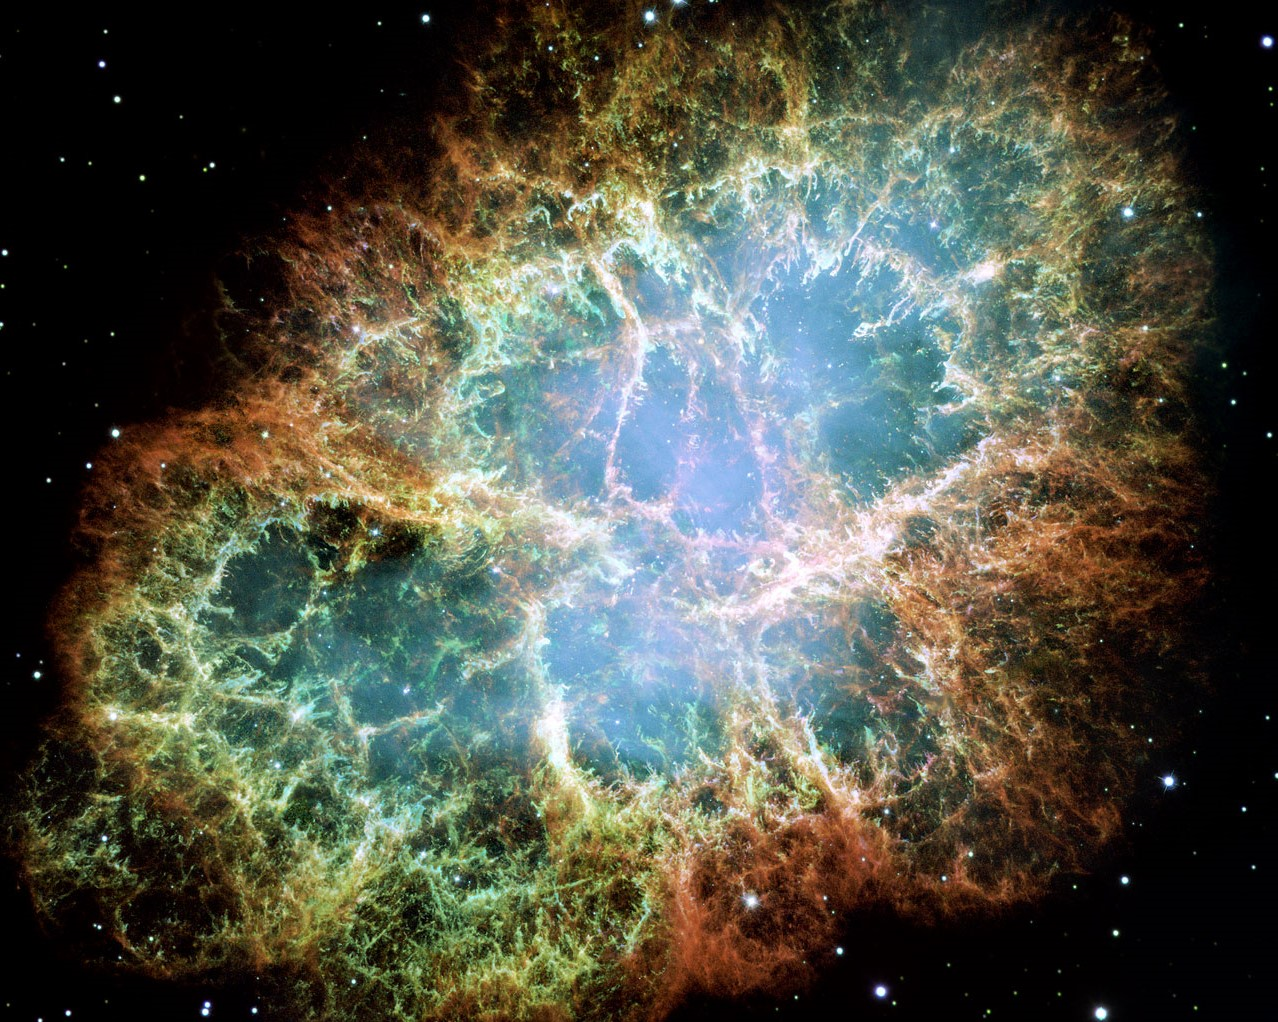
\includegraphics[width=\paperwidth, height =10cm]{../Crab.jpg}}
    \end{figure}
\end{titlepage}

%%%%%%%%%%%%%%%%%%%%%%%
\tableofcontents


%%%%%%%%%%%%%%%%%%%%%%%%%%%%%%%%%%%%% Part 1
\part{Theory}

%%%%%%%%%%%%%%%%%%%%%% Chapter 1.1
\chapter{The Wave Equation}


\section{The Schr\"{o}dinger Equation}

Consider a particle of mass $m$, constrained along the $x$ axis, subject to a specified force $F(x,t)$. In classical mechanics our goal is to determine the position function, $x(t)$. Once that is known, any other desired quantity such as velocity, momentum, and kinetic energy could be derivded. In deriving $x(t)$, we apply Newton's second law, $F = ma$ (for conservative systems). This together with the appropriate initial conditions fully specifies $x(t)$.

On the other hand, Quantum mechanics approaches this quite differently. In this case we're looking for a particle's \Emph{wave function}, $\Psi(x,t)$, and we get it by solving the \Emph{Schr\"{o}dinger equation}: \begin{equation*}
    \boxed{i\hbar\frac{\partial \Psi}{\partial t} = -\frac{\hbar^2}{2m}\frac{\partial^2\Psi}{\partial x^2}+V\Psi}
\end{equation*}
This plays the role logically analogous to Newton's second law; given suitable initial conditions, the Schr\"{o}dinger equation determines $\Psi(x,t)$ for all future $t$.


\section{Statistical Interpretation}

\begin{qst}
    What is this ``wave function," and what does it do for you once you've got it? How can we represent a particle with such an object?
\end{qst}


The answer is provided by Born's \Emph{statistical interpretation}, which says that $|\Psi(x,t)|^2$ gives the \Emph{probability of finding the particle at point $x$, at time $t$}, or more precisely \begin{equation*}
    \int_a^b|\Psi(x,t)|^2dx = \left\{\begin{array}{c} \text{probability of finding the particle} \\ \text{between $a$ and $b$, at time $t$}\end{array}\right\}
\end{equation*}
Probability in this case is the \Emph{area} under the graph $|\Psi|^2$. Note that the statistical intepretation introduces a kind of \Emph{indeterminacy} into quantum mechanics, for even if you know everything about the particle in terms of the theory (i.e. its wave function), you still cannot predict with certainty the outcome of a simple experiment to measure its position. This can be quite a disturbing outcome. For instance,

\begin{qst}
    If you do a measurement and find the position of a particle at some point, $A$, where was the particle just before you made the measurement?
\end{qst}

There are three main schools of thought which attempt to address this question: 

\begin{enumerate}
    \item The \Emph{realist} position: The particle was at $A$. Note that if this was true, then quantum mechanics is an incomplete theory. To the realist, indeterminacy is not a fact of nature, but a reflection of our ignorance.
    \item The \Emph{orthodox} position: The particle wasn't really anywhere. It was the act of measurement that forced it to ``choose." Jordan - ``Observations not only disturb what is to be measured, they produce it ... We compel [the particle] to assume a definite position." This is the \Emph{Copenhagen interpretation}, subscrobed by Bohr and his associates.
    \item The \Emph{agnostic} position: Refuse to answer. After all, what sense can there be in making assertions about the status of a particle before a measurement, when the only way of knowing whether you were right is precisely to make a measurement, in which case what you get is no longer ``before the measurement."
\end{enumerate}

In 1964, John Bell astonished the physics community by showing that it makes an observable difference whether the particle had a precise (though unknown) position prior to the measurement, or not. This eliminated agnosticism as a viable option, and made it an experimental question whether 1 or 2 is the correct choice; in the end it was the orthodox position that yielded the most sensical results. 

It is well agreed on that a repeated measurement on the same particle must return the same value. How does the orthodox interpretation account for this? We say that the wave function \Emph{collapses} upon measurement, to a spike at the point of measurement, although it soon spreads out again, in accordance with the Schr\"{o}dinger equation.


\section{Probability}

We begin our discussion of probability with a discrete probability distribution, $P(j)$, consisting of an at most countable number of probabilities. Normalization of probabilities implies that $$\sum_{j=0}^{\infty}P(j) = 1$$
Now, if $f$ is some function of the index variable $j$, we define the average or \Emph{expected value} of $f$ on $j$ to be \begin{equation*}
    \boxed{\langle f(j)\rangle = \sum_{j=0}^{\infty}f(j)P(j)}
\end{equation*}
A special case of this is the average value of the distribution: \begin{equation*}
    \boxed{\langle j\rangle = \sum_{j=0}^{\infty}jP(j)}
\end{equation*}
Now, how do we describe the spread of a distribution? We use the squared-mean-error, or \Emph{variance}, of the distribution: \begin{equation*}
    \boxed{\sigma^2 := \langle (j-\langle j\rangle)^2\rangle =: \langle (\Delta j)^2\rangle}
\end{equation*}
Here $\sigma$ itself is known as the \Emph{standard deviation}. It is useful to note the equality $$\sigma^2 = \langle(\Delta j)^2\rangle = \langle j^2\rangle - \langle j\rangle^2$$
so taking the square root we have $$\sigma = \sqrt{\langle j^2\rangle - \langle j \rangle^2}$$


We now move to working with probability distributions over continuous variables: variables ranging over intervals in $\R$. But, when making this switch we can no longer sensibly talk about the probability of an event occurring at a particular value of our continuous variable, and instead must discuss the probability that a result lies in some interval. Thus, we have the heuristic $$\left\{\begin{array}{c} \text{probability that an individual (chosen }\\ \text{at random) lies between $x$ and $(x+dx)$}\end{array}\right\} = \rho(x)dx$$
where the proportionality is known as our \Emph{probability density function}. 

\begin{defn}
    The probability that a measurement $X$ lies between points $a$ and $b$ in some finite interval for a continuous probability distribution with probability density $\rho(x)$ is \begin{equation*}
        P(a \leq X \leq b) = \int_a^b\rho(x)dx
    \end{equation*}
\end{defn}

By normalization conditions, we have that \begin{equation*}
    \int_{-\infty}^{\infty}\rho(x)dx = 1
\end{equation*}

\begin{defn}
    The expected value of a function $f$ with respect to a probability distribution with pdf $\rho(x)$ is $$\langle f(x)\rangle = \int_{-\infty}^{\infty}f(x)\rho(x)dx$$
\end{defn}

As in the discrete case, our variance for a continuous random variable is given by $$\sigma^2 := \langle (\Delta x)^2\rangle = \langle (x-\langle x\rangle)^2\rangle = \langle x^2\rangle - \langle x\rangle^2$$


\section{Normalization and the Wave Function}

Returning to the statistical interpretation of the wave function, and noting our discussions of probability in the previous section, we concur that the integral of $|\Psi|^2$ over all $x$ must be $1$ (the particle has to be somewhere) at any time $t$: $$\boxed{\int_{-\infty}^{\infty}|\Psi(x,t)|^2dx = 1}$$ Without this the statistical interpretation would be useless.

But, we must make sure that this normalization condition is consistent with the Schr\"{o}dinger equation which determines the wave function. But, recalling the Schr\"{o}dinger equation $$i\hbar\frac{\partial \Psi}{\partial t} = -\frac{\hbar^2}{2m}\frac{\partial^2\Psi}{\partial x^2}+V\Psi$$ if $\Psi(x,t)$ is a solution, $A\Psi(x,t)$ is as well for any $A \in \C$. Thus, we can pick this factor so that $\Psi(x,t)$ satisfies normalization. In some cases our solution gives an infinite integral, or even the $0$ integral if dealing with the trivial solution $\Psi \equiv 0$. Such \Emph{non-normalizable} solutions cannot represent particles, and must be rejected. Physically realizable states correspond to the \Emph{square-integrable} solutions to Schr\"{o}dinger's equation.

But, how do we ensure that once we normalize the wave function at $t = 0$, it will remain normalized indefinitely? This follows from the fact that the Schr\"{o}dinger equation has the property that it automatically preserves the normalization of the wave function - without this feature the Schr\"{o}dinger equation would be incompatible with the statistical intepretation, and the whole theory would crumble.

\begin{proof}[Proof of Time-Invariance of Normalization]
    To begin with, $$\frac{d}{dt}\int_{-\infty}^{\infty}|\Psi(x,t)|^2dx = \int_{-\infty}^{\infty}\frac{\partial}{\partial t}|\Psi(x,t)|^2dx$$ By the product rule $$\frac{\partial }{\partial t}|\Psi|^2 = \frac{\partial}{\partial t}(\Psi^*\Psi) = \Psi^*\frac{\partial\Psi}{\partial t}+\frac{\partial \Psi^*}{\partial t}\Psi$$ Now the Schr\"{o}dinger equation reads $$\frac{\partial \Psi}{\partial t} = \frac{i\hbar}{2m}\frac{\partial^2\Psi}{\partial x^2} - \frac{i}{\hbar}V\Psi$$ and hence taking the complex conjugate $$\frac{\partial \Psi^*}{\partial t} = -\frac{i\hbar}{2m}\frac{\partial^2\Psi^*}{\partial x^2} + \frac{i}{\hbar}V\Psi^*$$ so $$\frac{\partial}{\partial t}|\Psi|^2 = \frac{i\hbar}{2m}\left(\Psi^*\frac{\partial^2\Psi}{\partial x^2} - \frac{\partial^2\Psi^*}{\partial x^2}\Psi\right) = \frac{\partial}{\partial x}\left[\frac{i\hbar}{2m}\left(\Psi^*\frac{\partial \Psi}{\partial x} - \frac{\partial \Psi^*}{\partial x}\Psi\right)\right]$$
    Then we can evaluate our original integral using FTOC2 \begin{equation*}
        \frac{d}{dt}\int_{-\infty}^{\infty}|\Psi(x,t)|^2dx = \frac{i\hbar}{2m}\left(\Psi^*\frac{\partial \Psi}{\partial x} - \frac{\partial \Psi^*}{\partial x}\Psi\right)\Big\rvert_{-\infty}^{\infty}
    \end{equation*}
    But $\Psi(x,t)$ must go to zero as $x$ goes to infinity (otherwise the wave function would not be normalizable). It follows that $$\frac{d}{dt}\int_{-\infty}^{\infty}|\Psi(x,t)|^2dx = 0$$
    and hence the integral is constant.
\end{proof}


\section{Momentum}

For a particle in state $\Psi$, the expectation value of $x$ is \begin{equation*}
    \boxed{\langle x\rangle = \int_{-\infty}^{\infty}x|\Psi(x,t)|^2dx}
\end{equation*}
What does this mean? Note it does not mean that if you measure the position of one particle over and over again, $\int x|\Psi|^2dx$ is the average of the results you'll get. On the contrary, the first measurement, whose outcome is indeterminate, will collapse the wave function to a spike at the value actually obtained, and the subsequent measurements if they're performed quickly will simply repeat the same result. Rather, $\langle x\rangle$ is the average of measurements performed on particles all in the state $\Psi$, which means either you must find some way of returning the particle to its original state after each measurement, or else you have to prepare a whole \Emph{ensemble} of particles, each in the same state $\Psi$, and measure the positions of all of them. In short, the expectation value is the average of measurements on an ensemble of identically-prepared systems, not the average of repeated measurements on one and the same system.

As time moves, $\langle x\rangle$ may change since $\Psi$ is time dependent, so we might wish to look at how it changes: \begin{equation*}
    \frac{d\langle x\rangle}{dt} = \int_{-\infty}^{\infty}x\frac{\partial}{\partial t}|\Psi(x,t)|^2dx = \frac{i\hbar}{2m}\int_{-\infty}^{\infty}x\frac{\partial}{\partial x}\left(\Psi^*\frac{\partial\Psi}{\partial x} - \frac{\partial \Psi^*}{\partial x}\Psi\right)dx
\end{equation*}
This expression can be simplified with integration by parts to $$\frac{d\langle x\rangle}{dt} = -\frac{i\hbar}{2m}\int_{-\infty}^{\infty}\left(\Psi^*\frac{\partial \Psi}{\partial x} - \frac{\partial \Psi^*}{\partial x}\Psi\right)dx$$
Performing another integration by parts on the second term, we conclude $$\frac{d\langle x\rangle}{dt} = -\frac{i\hbar}{m}\int_{-\infty}^{\infty}\Psi^*\frac{\partial \Psi}{\partial x}dx$$

What does this mean? Note we are talking about a ``velocity" of the expectation value of $x$, which is \emph{not} the same as the velocity of the particle. Also, note it isn't clear yet if velocity makes sense in quantum mechanics - all we could ask for is the probability of getting a particular velocity. As we shall show later, the \Emph{expectation value of the velocity is equal to the time derivative of the expectation value of position}: $$\langle v\rangle = \frac{d\langle x\rangle}{dt} =  -\frac{i\hbar}{m}\int_{-\infty}^{\infty}\Psi^*\frac{\partial \Psi}{\partial x}dx$$

However, it is customary to work with \Emph{momentum}, $p = mv$, rather than velocity: \begin{equation*}
    \boxed{\langle p\rangle = m\frac{d\langle x\rangle}{dt} =  -i\hbar\int_{-\infty}^{\infty}\Psi^*\frac{\partial \Psi}{\partial x}dx}
\end{equation*}
We make the following observation on the forms of $\langle x\rangle$ and $\langle p\rangle$: \begin{align*}
    \langle x\rangle &= \int \Psi^*[x]\Psi dx \\
    \langle p\rangle &= \int\Psi^*[-i\hbar(\partial/\partial x)]\Psi dx
\end{align*}
We say that the \Emph{operator} $x$ ``represents" position, and the operator $-i\hbar(\partial/\partial x)$ ``represents" momentum.

The fact is all classical dynamical variables can be expressed in terms of position and momentum, and hence their corresponding variables can be derived: $$T = \frac{p^2}{2m}$$ and $$\mathbf{L} = \mathbf{r} \times \mathbf{p}$$
To calculate the expectation value of any such quantity $Q(x,p)$, we simply replace every $p$ by $-i\hbar(\partial/\partial x)$ and insert the resulting operator between $\Psi^*$ and $\Psi$, and integrate: \begin{equation*}
    \boxed{\langle Q(x,p)\rangle = \int \Psi^*\left[Q(x,-i\hbar \partial/\partial x)\right]\Psi dx}
\end{equation*}
For example the expectation value of the kinetic energy is $$\langle T\rangle = -\frac{\hbar^2}{2m}\int\Psi^*\frac{\partial^2\Psi}{\partial x^2}dx$$


\section{The Uncertainty Principle}

With any wave phenomenon (such as a wave on a string), the more packets (pulses) we observe the more well-defined the wavelength becomes, but the less well-defined a ``position" of the wave is, while the less packets we observe the more well-defined the position, but the less clear the wavelength. This applies to the quantum mechanical wave function as well. But, the wavelength of $\Psi$ is related to the momentum of the particle by the \Emph{de Broglie formula}: $$\boxed{p = \frac{h}{\lambda} = \frac{2\pi\hbar}{\lambda}}$$ Thus, a spread in wavelength corresponds to a spread in momentum, and our general observation now says that the more precisely determined a particle's position is, the less precisely determined its momentum. Quantitatively, $$\boxed{\sigma_x\sigma_p \geq \frac{\hbar}{2}}$$ where $\sigma_x$ is the standard deviation in $x$ and $\sigma_p$ is the standard deviation in $p$. This is Heisenberg's \Emph{uncertainty principle}.

Note what the uncertainty principle means: like position measurements, momentum measurements yield precise answers - the ``spread" here refers, as before, to the fact that measurements on identically prepared systems do not yield identical results. You can construct a state such that position measurements will be very close together (by making $\Psi$ a localized ``spike"), but you will pay a price: momentum measurements on this state will be widely scattered. Or you can prepare a state with a definite momentum by making $\Psi$ a long sinusoidal wave, but in that case position measurements will be widely scattered.


%%%%%%%%%%%%%%%%%%%%%% Chapter 1.2
\chapter{Time Independent Schr\"{o}dinger Equation}


\section{Stationary States}

\begin{qst}
    How do we get $\Psi(x,t)$?
\end{qst}

As was characterized in the first chapter, we need to solve the Schr\"{o}dinger equation: $$i\hbar\frac{\partial \Psi}{\partial t} = -\frac{\hbar^2}{2m}\frac{\partial^2\Psi}{\partial x^2} + V\Psi$$
for a specified potential $V(x,t)$. For this chapter we assume $V$ is independent of $t$. In this case we employ the method of \Emph{separation of variables}, looking for a solution of the form $$\Psi(x,t) = \psi(x)\varphi(t)$$
Although initially this will give us a really small subset of the solution space, the solutions we do obtain will be of great import, and we will hopefully be able to patch them together to obtain the most general solution.

Following this scheme we have $$\frac{\partial \Psi}{\partial t} = \psi\frac{d\varphi}{dt},\;\;\frac{\partial^2\Psi}{\partial^2x} = \frac{d^2\psi}{dx^2}\varphi$$
and the Schr\"{o}dinger equation reads $$i\hbar\psi\frac{d\varphi}{dt} = -\frac{\hbar^2}{2m}\frac{d^2\psi}{dx^2}\varphi+V\psi\varphi$$
or dividing through by $\psi\varphi$, $$i\hbar\frac{1}{\varphi}\frac{d\varphi}{dt} = -\frac{\hbar^2}{2m}\frac{d^2\psi}{dx^2}\frac{1}{\psi}+V$$
The left side is a function of $t$ along, and the right side is a function of $x$ alone. The only way this can possibly hold is if both sides are constant. Let us denote this separation constant by $E$: \begin{equation*}
    i\hbar\frac{1}{\varphi}\frac{d\varphi}{dt} = E,\;\;\implies\;\;\frac{d\varphi}{dt} = -\frac{iE}{\hbar}\varphi
\end{equation*}
and $$-\frac{\hbar^2}{2m}\frac{1}{\psi}\frac{d^2\psi}{dx^2}+V=E$$ or $$\boxed{-\frac{\hbar^2}{2m}\frac{d^2\psi}{dx^2} + V\psi = E\psi}$$
The first of these is easy to solve, with $\varphi = C\exp\left\{-\frac{iEt}{\hbar}\right\}$ being the general solution, but we can just absorb the constant into $\psi$ since we are considering the product $\varphi\psi$. Then $$\varphi(t) = e^{-iEt/\hbar}$$ The second equation is called the \Emph{time-independent Schr\"{o}dinger equation}; we now need $V(x)$ to go further.

\begin{rmk}
    Separable solutions are interesting for three reasons:\begin{itemize}
        \item[(i)] They correspond to \Emph{stationary states}. Although the wave-function itsefl, $$\Psi(x,t) = \psi(x)e^{-iEt/\hbar}$$ depends on $t$, the probability density, $$|\Psi(x,t)|^2 = \Psi^*\Psi = |\psi(x)|^2$$ is indepdent of time. The same result occurs when calculating the expectation value of any dynamical variable: $$\langle Q(x,p)\rangle = \int\psi^*\left[Q\left(x,-i\hbar\frac{d}{dx}\right)\right]\psi dx$$
            In particular, $\langle x\rangle$ is constant, and hence $\langle p \rangle = m\frac{d\langle x\rangle}{dt} = 0$ (nothing ever happens in a stationary state)
        \item[(ii)] They are states of \emph{definite total energy}. The Hamiltonian operator, obtained from $H(x,p) = \frac{p^2}{2m}+V(x)$ obtained from the substitution $p\rightarrow -i\hbar(\partial/\partial x)$, is therefore $$\hat{H} = -\frac{\hbar^2}{2m}\frac{\partial^2}{\partial x^2} + V(x)$$
            Thus, the time-independent Schr\"{o}dinger equation can be written $$\hat{H}\psi = E\psi$$
            and the expecation value of the total energy is $$\langle H\rangle = \int \psi^*\hat{H}\psi dx = E\int|\psi|^2dx = E\int|\Psi|^2dx = E$$
            Moreover, $\hat{H}^2\psi = \hat{H}(E\psi) = E\hat{H}\psi = E^2\psi$, and hence $$\langle H^2\rangle = \int\psi^*\hat{H}^2\psi dx = E^2\int|\psi|^2dx = E^2$$ so the variance of $H$ is $$\sigma_H^2 = \langle H^2\rangle - \langle H\rangle^2 = 0$$
            Consequently, a separable solution has the property that every measurement of the total energy is certain to return the value $E$.
        \item[(iii)] The general solution is spanned by the separable solutions (i.e. is a linear combination of them). Indeed, since the time-independent solution is linear in $\psi$, every linear combination of solutions is again a solution. It so happens that every solution to the time-dependent Schr\"{o}dinger equation can be written in the form $$\Psi(x,t) = \sum_{n=1}^{\infty}c_n\psi_n(x)e^{-iE_nt/\hbar}$$ for suitable constants, $c_1,c_2,...$, and where $\psi_n$ is the time-independent solution with corresponding energy $E_n$.
    \end{itemize}
\end{rmk}

As we shall show later, the coefficients in the expansion of $\Psi(x,t)$ in terms of the $\psi_n(x)$ correspond to probabilities. In particular, $|c_n|^2$ is the probability that a measurement of the energy would return the value $E_n$. A competent measurement will always yield one of the ``allowed" values, and $|c_n|^2$ is the probability of getting a particular value $E_n$. Of course, as we shall later show, $\sum_{n=1}^{\infty}|c_n|^2 = 1$, and the expectation value of the energy must be $$\langle H\rangle =\sum_{n=1}^{\infty}|c_n|^2E_n$$
Notice that because the constants are independent of time, so too is the probability of getting a particular energy, and a fortiori, the expectation value of $H$. These are manifestations of \Emph{energy conservation} in quantum mechanics.




\section{The Infinite Square Well}


Suppose we consider a system with potential $$V(x) = \left\{\begin{array}{lc} 0, & 0 \leq x \leq a \\ \infty, & \text{otherwise} \end{array}\right.$$
A particle in this potential is completely free, except at the two ends ($x = 0$ and $x = a$), where an infinite force prevents it from escaping. 

Outside the well, $\phi(x) = 0$ (the probability of finding the particle there is zero). Inside the well, where $V = 0$, the time-independent Schr\"{o}dinger equation reads $$-\frac{\hbar^2}{2m}\frac{d^2\psi}{dx^2} = E\psi$$
or $\frac{d^2\psi}{dx^2} = -k^2\psi$, where $k \equiv \frac{\sqrt{2mE}}{\hbar}$, assuming $E \geq 0$. This is the equation of the classical \Emph{simple harmonic oscillator}, the general solution of which is $$\psi = A\sin kx + B \cos kx$$ where $A$ and $B$ are arbitrary constants. Typically $A$ and $B$ are determined by boundary conditions. 

Ordinarily we require $\psi$ and $d\psi/dx$ to be continuous at the boundary, but where the potential goes to infinity only the first of these need apply. (note $\Psi(x,t)$ need not be a continuous function of $x$) Continuity equates to $\psi(0) = \psi(a) = 0$. This tells us that $B = \psi(0) = 0$, and hence $\psi(x) = A\sin kx$. Further, $0 = \psi(a) = A\sin ka$, so either $A = 0$, or $ka = \pi n$, for $n \in \N$. But $k = 0$ is not interesting as that would imply $\psi(x) = 0$, and by oddness of the sine function positives and negatives are inconsequential, so the distinct solutions are \begin{equation*}
    k_n = \frac{n\pi}{a}, \;\; n =1,2,3,...
\end{equation*}
Thus, the possible values of $E$ are \begin{equation*}
    \boxed{E_n = \frac{\hbar^2k_n^2}{2m} = \frac{n^2\pi^2\hbar^2}{2ma^2}}
\end{equation*}
and we arrive at a result with quantized energies. To find $A$ we normalize $\psi$: \begin{equation*}
    \int_0^a|A|^2\sin^2(kx)dx = |A|^2\frac{a}{2} = 1,\;\text{ so }\;|A|^2 = \frac{2}{a}
\end{equation*}
For simplicity we take the positive real root, $A = \sqrt{2/a}$. Inside the well, the solutions are \begin{equation*}
    \boxed{\psi_n(x) = \sqrt{\frac{2}{a}}\sin\left(\frac{n\pi}{a}x\right)}
\end{equation*}
The state corresponding to $n = 1$, with the lowest energy, is called the \Emph{ground state}, while all other states are called \Emph{excited states}.

\begin{prop}
    The collection of eigenfunctions $\psi_n(x)$ satisfy the following properties: \begin{itemize}
        \item They are alternately even and odd, with respect to the center of the well.
        \item Each successive state has one more \Emph{node} (zero-crossing/root) (note we don't count the endpoints, so $\psi_1$ has none)
        \item They are mutually orthogonal with respect to the standard inner product $$\int\psi_m(x)^*\psi_n(x)dx = \delta_{mn}$$
        \item They are \Emph{complete}, in the sense that any other function can be expressed as a linear combination of them: $$f(x) = \sum_{n=1}^{\infty}c_n\psi_n(x) = \sqrt{\frac{2}{a}}\sum_{n=1}^{\infty}c_n\sin\left(\frac{n\pi}{a}x\right)$$
            (this is simply a Fourier Series with odd periodic expansion for $f(x)$). We can compute the Fourier coefficients using the standard method for complete orthonormal sets: $$c_m = \braket{\psi_m}{f} = \int\psi_m(x)^*f(x)dx$$
    \end{itemize}
\end{prop}


The first property is true whenever the potential is symmetric, the second is universal for eigenfunctions, orthogonality is quite general, and completeness holds for all potentials often encountered physically.

The stationary states of the infinite square well are then $$\Psi_n(x,t) = \sqrt{\frac{2}{a}}\sin\left(\frac{n\pi}{a}x\right)e^{-i(n^2\pi^2\hbar/2ma^2)t}$$ Then the most general solution is of the form $$\Psi(x,t) = \sum_{n=1}^{\infty}c_n\sqrt{\frac{2}{a}}\sin\left(\frac{n\pi}{a}x\right)e^{-i(n^2\pi^2\hbar/2ma^2)t}$$
By completeness of the $\psi$'s, we may choose appropriate $c_n$ such that $\Psi(x,0) = \sum_{n=1}^{\infty}c_n\psi_n(x)$ given any initial conditions. These are precisely the coefficients that hold in general.


\section{The Harmonic Oscillator}


Recall from classical mechanics for formula known as \Emph{Hooke's law} for classical harmonic oscillators of mass $m$ and force constant $k$, $F = -kx = m\frac{d^2x}{dt^2}$, and the solution $x(t) = A\sin(\omega t) + B\cos(\omega t)$, where $\omega \equiv \sqrt{\frac{k}{m}}$ is the angular frequency of oscillation. The associated potential, $V(x) = \frac{1}{2}kx^2$, has graph a simple parabola.

We can generalize this to potentials about their minima. If $x_0$ is a minima of a potential $V$, $V'(x_0) = 0$ and we can adjust $V$ be a constant such that $V(x_0)$, so its Taylor series takes the form $$V(x) = \frac{1}{2}V''(x_0)(x-x_0)^2 + O((x-x_0)^3)$$
sufficiently close to the minima $V(x) \approx \frac{1}{2}V''(x_0)(x-x_0)^2$, which describes simple harmonic oscillation about the minima with spring constant $k = V''(x_0)$. 

Our problem now is to solve the Schr\"{o}dinger equation for the potential $$V(x) = \frac{1}{2}m\omega^2x^2$$
where $\omega = \sqrt{\frac{k}{m}}$. It suffices to find separable solutions, and so solve the time-independent Schr\"{o}dinger equation: $$-\frac{\hbar^2}{2m}\frac{d^2\psi}{dx^2} + \frac{1}{2}m\omega^2x^2\psi = E\psi$$
We solve this problem in two ways.

\subsection{Ladder Operator Technique}

To begin, we rewrite the time-independent Schr\"{o}dinger equation as $$\frac{1}{2m}\left[\hat{p}^2 + (m\omega x)^2\right]\psi = E\psi$$
using $\hat{p} = -i\hbar\frac{\partial}{\partial x}$. The idea is to factor the Hamiltonian. But, as we are dealing with distinct operators $\hat{p}$ and $\hat{x}$, we don't necessarily have commutativity as we do for complex numbers, so we need to proceed cautiously. 

\begin{defn}
    We define the \Emph{ladder operators} to be $$\hat{a}_+ := \frac{1}{\sqrt{2\hbar m\omega}}(-i\hat{p} + m\omega x),\;\;\hat{a}_- := \frac{1}{\sqrt{2\hbar m\omega}}(+i\hat{p}+m\omega x)$$
\end{defn}
What are the products of these operators? $$\hat{a}_-\hat{a}_+ = \frac{1}{2\hbar m\omega}\left[\hat{p}^2+i\hat{p}m\omega x - im\omega x\hat{p} + (m\omega x)^2\right] = \frac{1}{2\hbar m\omega}\left[\hat{p}^2+(m\omega x)^2 - im\omega(x\hat{p} - \hat{p}x)\right]$$
and $$\hat{a}_+\hat{a}_- = \frac{1}{2\hbar m\omega}\left[\hat{p}^2-i\hat{p}m\omega x + im\omega x\hat{p} + (m\omega x)^2\right] = \frac{1}{2\hbar m\omega}\left[\hat{p}^2+(m\omega x)^2 + im\omega(x\hat{p} - \hat{p}x)\right]$$
In both cases we have the term $(x\hat{p}-\hat{p}x)$, the \Emph{commutator} of $x$ and $\hat{p}$, denoted $[\hat{x},\hat{p}]$, for $\hat{x} = x$. In this notation $$\hat{a}_-\hat{a}_+ = \frac{1}{2\hbar m\omega}[\hat{p}^2+(m\omega x^2)] - \frac{i}{2\hbar}[\hat{x},\hat{p}]$$
and $$\hat{a}_+\hat{a}_- = \frac{1}{2\hbar m\omega}[\hat{p}^2+(m\omega x^2)] + \frac{i}{2\hbar}[\hat{x},\hat{p}]$$
Let $f(x)$ be an arbitrary function in the Hilbert space. It follows that \begin{align*}
    [\hat{x},\hat{p}]f(x) &= \left[x(-i\hbar)\frac{d}{dx}(f) - (-i\hbar)\frac{d}{dx}(xf)\right] \\
    &= -i\hbar\left[xf'(x) - xf'(x) - f(x)\right] = i\hbar f(x)
\end{align*}
so $$[\hat{x},\hat{p}] = i\hbar$$
this is often called the \Emph{canonical commutation relation}. With this equation, going back we have $$\hat{a}_-\hat{a}_+ = \frac{1}{\hbar \omega}\hat{H} + \frac{1}{2},\;\;\hat{a}_+\hat{a}_- = \frac{1}{\hbar \omega}\hat{H} - \frac{1}{2}$$
so $$\hat{H} = \hbar\omega\left(\hat{a}_-\hat{a}_+ - \frac{1}{2}\right) = \hbar \omega\left(\hat{a}_+\hat{a}_- + \frac{1}{2}\right)$$
Observe that $[\hat{a}_-,\hat{a}_+] = 1$. Then the Schr\"{o}dinger equation for the harmonic oscillator can be written $$\hbar \omega \left(\hat{a}_{\pm}\hat{a}_{\mp}\pm\frac{1}{2}\right)\psi = E\psi$$

\begin{prop}
    If $\psi$ satisfies the Schr\"{o}dinger equation with energy $E$, then $\hat{a}_{\pm}\psi$ satisfies the Schr\"{o}dinger equation with energy $E\pm\hbar\omega$.
\end{prop}
\begin{proof}
    Observe \begin{align*}
        \hat{H}(\hat{a}_{\pm}\psi) = \hbar\omega\left(\hat{a}_{\pm}\hat{a}_{\mp} \pm \frac{1}{2}\right)(\hat{a}_{\pm}\psi) \\
        &= \hbar \omega\hat{a}_{\pm}\left(\hat{a}_{\mp}\hat{a}_{\pm} \pm1 \mp\frac{1}{2}\right)\psi \\
        &= \left(E \pm \hbar\omega\right)(\hat{a}_{\pm}\psi)
    \end{align*}
    so $$\hat{H}(\hat{a}_+\psi) = (E + \hbar\omega)(\hat{a}_+\psi),\;\;\hat{H}(\hat{a}_-\psi) = (E-\hbar\omega)(\hat{a}_-\psi)$$
\end{proof}

We call $\hat{a}_+$ the \Emph{raising operator} and $\hat{a}_-$ the \Emph{lowering operator} for this reason.

\begin{qst}
    What if I apply the lowering operator repeatedly?
\end{qst}

At some point the machine must fail, but how can that happen? We know $\hat{a}_-\psi$ is a new solution, but there is no guarantee it will be normalizable-it may be zero, or have infinite integral. In practice it is the former. There exists $\psi_0$ such that $\psi_0 \neq 0$, but $$\hat{a}_-\psi_0 = 0$$
We can determine $\psi_0(x)$ by $$\frac{1}{\sqrt{2\hbar m\omega}}\left(\hbar\frac{d}{dx} + m\omega x\right)\psi_0 = 0$$
or $\frac{d\psi_0}{dx} = -\frac{m\omega}{\hbar}x\psi_0$. By separation of variables, $$\psi_0(x) = Ae^{-\frac{m\omega}{2\hbar}x^2}$$
and normalizing $$1 = |A|^2\int_{-\infty}^{\infty}e^{-m\omega x^2/\hbar}dx = |A|^2\sqrt{\frac{\pi\hbar}{m\omega}}$$
so $A^2 = \sqrt{m\omega/\pi\hbar}$, and hence \begin{equation*}
    \boxed{\psi_0(x) = \left(\frac{m\omega }{\pi\hbar}\right)^{1/4}e^{-\frac{m\omega}{2\hbar}x^2}}
\end{equation*}
To determine the energy, we plug into the Schr\"{o}dinger equation, $\hbar\omega(\hat{a}_+\hat{a}_- +1/2)\psi_0 = E_0\psi_0$, which implies $$E_0 = \frac{1}{2}\hbar\omega$$
This is the \Emph{ground state} energy of the quantum harmonic oscillator. Then, for each $n \in \N$, $$\psi_n(x) = A_n(\hat{a}_+)^n\psi_0(x),\;\text{ with }\;E_n = \left(n+\frac{1}{2}\right)\hbar\omega$$

We can also use this to obtain normalization. Note $\hat{a}_{\pm}\psi_n \propto \psi_{n\pm 1}$, so $\hat{a}_+\psi_n = c_n\psi_{n+1}$ and $\hat{a}_-\psi_n = d_n\psi_{n-1}$.

\begin{prop}
    $\hat{a}_{\mp}$ is the \Emph{hermitian conjugate}, or \Emph{adjoint} of $\hat{a}_{\pm}$.
\end{prop}
\begin{proof}
    Observe \begin{equation*}
        \int_{-\infty}^{\infty}f^*\cdot(\hat{a}_{\pm}g)dx = \frac{1}{\sqrt{2\hbar m\omega}}\int_{-\infty}^{\infty}f^*\cdot \left(\mp \hbar\frac{d}{dx} + m\omega x\right)gdx
    \end{equation*}
    and integration by parts takes $\int f^*\cdot (dg/dx)dx$ to $-\int(df/dx)^*gdx$. So \begin{align*}
        \int_{-\infty}^{\infty}f^*\cdot (\hat{a}_{\pm}g)dx &= \frac{1}{\sqrt{2\hbar m\omega}}\int_{-\infty}^{\infty}\left[\left(\pm\hbar\frac{d}{dx} + m\omega x\right)f\right]^*gdx \\
        &= \int_{-\infty}^{\infty}(\hat{a}_{\mp}f)^*gdx
    \end{align*}
\end{proof}

It follows that $$\braket{\hat{a}_{\pm}\psi_n}{\hat{a}_{\pm}\psi_n} = \braket{\hat{a}_{\mp}\hat{a}_{\pm}\psi_n}{\psi_n}$$
Using $\hat{a}_+\hat{a}_-\psi_n = n\psi_n$ and $\hat{a}_-\hat{a}_+\psi_n = (n+1)\psi_n$, so $$\braket{\hat{a}_+\psi_n}{\hat{a}_+\psi_n} = (n+1) = |c_n|^2$$ and $$\braket{\hat{a}_-\psi_n}{\hat{a}_-\psi_n} = n = |d_n|^2$$
Thus, \begin{equation*}
    \boxed{\hat{a}_+\psi_n = \sqrt{n+1}\psi_{n+1},\;\;\hat{a}_-\psi_n = \sqrt{n}\psi_{n-1}}
\end{equation*}
In general, $$\boxed{\psi_n = \frac{1}{\sqrt{n!}}(\hat{a}_+)^n\psi_0}$$
As in the square well-case, we have orthonormality - this follows from the fact that these $\psi_n$ are eigenfunctions of $\hat{a}_+\hat{a}_-$, which is Hermitian being the product of an operator and its adjoint, with eigenvalue $n$, so for $\psi_n,\psi_m$, $m \neq n$, the distinct eigenvalues (with the discrete spectra) imply orthonormality of the result. Then we can expand $\Psi(x,0)$ as a linear combination of stationary states using Fourier coefficients $c_n$. As before, $|c_n|^2$ is the probability that a measurement of the energy would yield the value $E_n$.





\section{The Free Particle}


We now consider the free particle ($V(x) = 0$ everywhere). The time-independent Schr\"{o}dinger equation now reads \begin{equation*}
    -\frac{\hbar^2}{2m}\frac{d^2\psi}{dx^2} = E\psi
\end{equation*}
or \begin{equation*}
    \frac{d^2\psi}{dx^2} = -k^2\psi,\;\text{ where }k := \frac{\sqrt{2mE}}{\hbar}
\end{equation*}
Writing the solution in exponential form we have $$\psi(x) = Ae^{ikx} + Be^{-ikx}$$
Since there are no boundary conditions, the free particle can carry any positive energy. Tacking on the standard time dependence. $\exp(-iEt/\hbar)$, \begin{equation*}
    \Psi(x,t) = Ae^{ik\left(x-\frac{\hbar k}{2m}t\right)} + Be^{-ik\left(x+\frac{\hbar k}{2m}t\right)}
\end{equation*}
Note any function of $x$ and $t$ that depends on these variables in the special combination $x\pm vt$ for some constant $v$ represents a wave of unchanging shape, traveling in the $\mp x$ direction at speed $v$. You can think of it as a fixed point on the waveform (for example a maxima or minima) corresponding to the argument being constant, $x\pm vt = $ const, or equivalently $x = \mp vt + $ const.
Thus, the first term represents a wave traveling to the right while the second represents a wave traveling to the left.

We could also write this as \begin{equation*}
    \Psi_k(x,t) = Ae^{i\left(kx - \frac{\hbar k^2}{2m}t\right)}
\end{equation*}
where now $k$ can be negative: \begin{equation*}
    k := \left\{\begin{array}{cc} \frac{\sqrt{2mE}}{\hbar} & \text{traveling to the right} \\ -\frac{\sqrt{2mE}}{\hbar} & \text{traveling to the left} \end{array}\right.
\end{equation*}

The `stationary states' of the free particle are propagating waves with wavelength $\lambda = 2\pi/|k|$, and according to the de Broglie formula carrying momentum $$p = \hbar k$$
The speed of these waves (the coefficient of $t$) is \begin{equation*}
    \boxed{v_{quantum} = \frac{\hbar|k|}{2m} = \sqrt{\frac{E}{2m}}}
\end{equation*}
On the other hand, the \emph{classical} speed of a free particle with energy $E$ is given by $E = \frac{1}{2}mv^2$ (pure kinetic, since $V = 0$), so $$v_{classical} = \sqrt{\frac{2E}{m}} = 2v_{quantum}$$
We'll return to this discrepancy in a moment. First we must address the following issue:
\begin{equation*}
    \text{\emph{This wave function is not normalizable}}
\end{equation*}
\begin{equation*}
    \int_{-\infty}^{\infty}\Psi^*_k\Psi_kdx = |A|^2\int_{-\infty}^{\infty}dx = |A|^2(\infty)
\end{equation*}
Consequently, the separable solutions do not represent physically realizable states in this case. A free particle cannot exist in a stationary state, or to put it another way, there is no such thing as a free particle with a definite energy.

But, we can still construct the general colution to the time-dependent Schr\"{o}dinger equation as a linear combination of separable solutions, only this time it is over a continuous variable $k$:\begin{equation*}
    \boxed{\Psi(x,t) = \frac{1}{\sqrt{2\pi}}\int_{-\infty}^{\infty}\phi(k)e^{i\left(kx-\frac{\hbar k^2}{2m}t\right)}dk}
\end{equation*}
For appropriate $\phi(k)$ this can be normalized. But it necessarily carries a range of $k$s, and hence a range of energies and speeds. We call it a \Emph{wave packet}.

In general we are given $\Psi(x,0)$, and want to find $\Psi(x,t)$. For a free particle the only question is how to determined $\phi(k)$ so as to match the initial wave function: \begin{equation*}
    \Psi(x,0) = \frac{1}{\sqrt{2\pi}}\int_{-\infty}^{\infty}\phi(k)e^{ikx}dk
\end{equation*}
This is classically solved by the Inverse Fourier transform: \begin{equation*}
    \boxed{\phi(k) = \frac{1}{\sqrt{2\pi}}\int_{-\infty}^{\infty}\Psi(x,0)e^{-ikx}dx}
\end{equation*}

The issue of $\Psi_k(x,t)$ not traveling at the classical speed vanishes when we realize it is not a physically realizable state. Nonetheless, we can still derive information about the particle velocity from the wave function. Note a wave packet is a superposition of sinusoidal functions whose amplitude is modulated by $\phi$ (ripples contained in an envolope). What corresponds to the particle velocity is not the speed of the individual ripples (the \Emph{phase velocity}), but rather the speed of the envelope (the \Emph{group velocity}). Depending on the wave the group velocity can be greater than, less than, or equal to the phase velocity. For a wave packet of the generic form \begin{equation*}
    \Psi(x,t) = \frac{1}{\sqrt{2\pi}}\int_{-\infty}^{\infty}\phi(k)e^{i(kx-\omega t)}dk
\end{equation*}
where $\omega = \hbar k^2/2m$ is the \Emph{dispersion relation} in our case. Assume $\phi(k)$ is narrowly peaked about some particular value $k_0$ (for broad spreads in $k$, the wave packets change shape rapidly so there isn't necessarily a well defined notion of a ``group"). We Taylor expand about $k_0$, giving $\omega(k)\approx \omega_0 + \omega_0'(k-k_0)$, where $\omega_0' = \omega'(k_0)$. Changing variables to $s\equiv k-k_0$, we have \begin{align*}
    \Psi(x,t) &\approx \frac{1}{\sqrt{2\pi}}\int_{-\infty}^{\infty}\phi(k_0+s)e^{i[(k_0+s)x-(\omega_0+\omega_0')t]}ds \\
    &= \frac{1}{\sqrt{2\pi}}e^{i(k_0x-\omega_0t)}\int_{-\infty}^{\infty}\phi(k_0+s)e^{is(x-\omega_0't)}ds
\end{align*}
The term in front is a sinusoidal wave (the ripples), traveling at speed $\omega_0/k_0$. It is modulated by the integral (the envolope), which is a function of $x-\omega_0't$, and therefore propagates at the speed $\omega_0'$. Thus the phase velocity is \begin{equation*}
    \boxed{v_{phase} = \frac{\omega}{k}}
\end{equation*}
while the group velocity is \begin{equation*}
    \boxed{v_{group} = \frac{d\omega}{dk}}
\end{equation*}
both evaluated at $k_0$.

In our case of $\omega = \hbar k^2/2m$, this gives $\omega/k = \hbar k/2m$ and $d\omega/dk = \hbar k/m$, confirming that the group velocity of the wave packet matches the classical particle velocity.



\section{The Delta-Function Potential}

\subsection{Bound States and Scattering States}

Recall in classical mechanics that if the energy of a particle is less than the potential at some points, it is in a \Emph{bound state}, and oscillates between the turning points at which $E = V(x)$. When this is not the case and the particle is free to fly either to plus or minus infinity, or both, it is said to be in a \Emph{scattering state}. 

In quantum mechanics the particle may ``leak" through a finite potential barrier, even if it is classically bound, exhibiting the phenomena of \Emph{tunneling}, so all that matters is the potential at infinity: \begin{equation*}
    \left\{\begin{array}{c} E < V(-\infty)\text{ and }V(+\infty)\implies\text{ bound state} \\ E>V(-\infty)\text{ or }V(+\infty)\implies\text{ scattering state}\end{array}\right.
\end{equation*}


\subsection{The Delta-Function Well}

\begin{defn}
    The \Emph{dirac delta function} is characterized by $\delta(x) = 0, x\neq 0$ and $\delta(x) = \infty$ if $x = 0$, with $$\int_{-\infty}^{\infty}\delta(x)dx = 1$$
\end{defn}

Let's consider a potential of the form \begin{equation*}
    V(x) = -\alpha\delta(x)
\end{equation*}
where $\alpha$ is some positive constant. The Schr\"{o}dinger equation reads \begin{equation*}
    -\frac{\hbar^2}{2m}\frac{d^2\psi}{dx^2}-\alpha\delta(x)\psi = E\psi
\end{equation*}
It yields both bound states $(E < 0)$, and scattering states $(E > 0)$.

First consider bound states. In the region $x < 0$, $V(x) = 0$ so \begin{equation*}
    \frac{d^2\psi}{dx^2} = -\frac{2mE}{\hbar^2}\psi = \kappa^2\psi
\end{equation*}
for $\kappa = \frac{\sqrt{-2mE}}{\hbar}$, with general solution \begin{equation*}
    \psi(x) = Ae^{-\kappa x}+Be^{\kappa x}
\end{equation*}
As it must go to zero when $x\rightarrow -\infty$, we must have $A = 0$, so $$\psi(x) = Be^{\kappa x}, (x < 0)$$
Similarly, for $x > 0$ $V(x)$ is again $0$ so $$\psi(x) = Fe^{-\kappa x}, (x > 0)$$
We now apply the standard boundary conditions: \begin{equation*}
    \boxed{\left\{\begin{array}{ccc} 1. & \psi & \text{ is always continuous} \\ 2. & d\psi/dx & \text{ is continuous except at points where $V = \infty$} \end{array}\right.}
\end{equation*}
The first condition tells us $F = B$. The second condition we can't apply. To look at the discontinuity of $d\psi/dx$ at $0$ we integrate the Schr\"{o}dinger equation from $-\epsilon$ to $+\epsilon$, and take the limit \begin{equation*}
    -\frac{\hbar^2}{2m}\int_{-\epsilon}^{+\epsilon}\frac{d^2\psi}{dx^2}dx + \int_{-\epsilon}^{+\epsilon}V(x)\psi(x)dx = E\int_{-\epsilon}^{+\epsilon}\psi(x)dx
\end{equation*}
In the limit as $\epsilon \rightarrow 0$, \begin{equation*}
    \Delta\left(\frac{d\psi}{dx}\right) :=\lim\limits_{\epsilon\rightarrow 0}\left(\frac{\partial\psi}{\partial x}\Bigg\rvert_{+\epsilon} - \frac{\partial \psi}{\partial x}\Bigg\rvert_{-\epsilon}\right) = \frac{2m}{\hbar^2}\lim\limits_{\epsilon\rightarrow 0}\int_{-\epsilon}^{+\epsilon}V(x)\psi(x)dx
\end{equation*}
By definition of the $\delta$ function we have that \begin{equation*}
    \boxed{\Delta \left(\frac{d\psi}{dx}\right) = -\frac{2m\alpha}{\hbar^2}\psi(0)}
\end{equation*}
We can also compute $d\psi/dx\vert_+ = -B\kappa$ and $d\psi/dx\vert_- = +B\kappa$, so $\Delta(d\psi/dx) = -2B\kappa$. Thus, equating these terms we have \begin{equation*}
    \kappa = \frac{m\alpha}{\hbar^2}
\end{equation*}
and the allowed energy is $$E = -\frac{m\alpha^2}{2\hbar^2}$$
Finally, normalizing $\psi$ we have $\frac{|B|^2}{\kappa} = 1$, so \begin{equation*}
    B = \sqrt{\kappa} = \frac{\sqrt{m\alpha}}{\hbar}
\end{equation*}
Evidently we have exactly one bound state:\begin{equation*}
    \boxed{\psi(x) = \frac{\sqrt{m\alpha}}{\hbar}e^{-m\alpha|x|/\hbar^2};\;\;E=-\frac{m\alpha^2}{2\hbar^2}}
\end{equation*}


Now we address scattering states where $E > 0$. For $x < 0$ and $x > 0$ the equation reads $\frac{d^2\psi}{dx^2} = -k^2\psi$ for $\psi = \frac{\sqrt{2mE}}{\hbar}$, with general solutions $\psi(x) = Ae^{ikx} +Be^{-ikx}$ and $\psi(x) = Fe^{ikx} + Ge^{-ikx}$ for $x < 0$ and $x > 0$ respectively. The continuity at $x = 0$ requires $$F+G = A+B$$
For the derivatives we have $d\psi/dx\vert_+ = ik(F-G)$ and $d\psi/dx\vert_- = ik(A-B)$, so $\Delta(d\psi/dx) = ik(F-G-A+B)$. Meanwhile $\psi(0) = A+B$, so the second boundary condition says \begin{equation*}
    ik(F-G-A+B) = -\frac{2m\alpha}{\hbar^2}(A+B)
\end{equation*}
or more compactly \begin{equation*}
    F-G = A(1+2i\beta)-B(1-2i\beta),\text{ where }\beta :=\frac{m\alpha}{\hbar^2k}
\end{equation*}
We now have two equations and four unknowns (five counting $k$). Note this is not a normalizable state. Instead of proceeding with this, we look at the physical significance of the constants. Combining with the wiggle factor we note $A$ is the amplitude of a wave coming in from the left, $B$ is the amplitude of a wave returning to the left, $F$ is the amplitude of a wave traveling off to the right, and $G$ is the amplitude of a wave coming in from the right. In typical scattering we investigate a source from one direction. Let's say it is coming in from the left. In that case the amplitude of the wave coming in from the right will be zero, $G = 0$. $A$ is the amplitude of the \Emph{incident wave}, $B$ is the amplitude of the \Emph{reflected wave}, and $F$ is the amplitude of the \Emph{transmitted wave}. Solving our equations for $B$ and $F$ we find \begin{equation*}
    B = \frac{i\beta}{1-i\beta}A,\;\;F = \frac{1}{1-i\beta}A
\end{equation*}

The probability of finding a particle at a specific location is given by $|\Psi|^2$, so the relative probability that an incident particle will be reflected back is \begin{equation*}
    R = \frac{|B|^2}{|A|^2} = \frac{\beta^2}{1+\beta^2}
\end{equation*}
called the \Emph{reflection coefficient}. Meanwhile, the probability that a particle will continue right on through it the \Emph{transmission coefficient}:\begin{equation*}
    T = \frac{|F|^2}{|A|^2} = \frac{1}{1+\beta^2}
\end{equation*}
Note the sum equals $1$: $R+T = 1$. Written explicitly we have \begin{equation*}
    \boxed{R=\frac{1}{1+(2\hbar^2E/m\alpha^2)},\;\;T=\frac{1}{1+(m\alpha^2/2\hbar^2E)}}
\end{equation*}

As $E$ increases, so does $T$ (the probability of transmission). But note that this is all analysis of the stationary states, which are not normalizable and hence do not actually represent physical particles. If we flip the well into a barrier the bound state is killed, but the reflection and transmission coefficients remain unchanged.


\section{The Finite Square Well}

Now we consider the example of a finite square well: \begin{equation*}
    V(x) = \left\{\begin{array}{cc} -V_0 & -a\leq x \leq a \\ 0 & |x| > 0 \end{array}\right.
\end{equation*}
where $V_0 > 0$ is constant. This admits both bound ($E < 0)$ and scattering $(E > 0)$ states.

Let us consider $E < 0$ first. For $x < -a$ we are in a similar solution to the infinite case with $\psi(x) = Be^{\kappa x}$ where $\kappa = \frac{\sqrt{-2mE}}{\hbar}$. In the region $-a < x < a$, $V(x) = -V_0$, and the wave equation reads \begin{equation*}
    \frac{d^2\psi}{dx^2} = -l^2\psi
\end{equation*}
where $l = \frac{\sqrt{2m(E+V_0)}}{\hbar}$. Although $E < 0$, we require $E > -V_0$, so $E+V_0 > 0$. The general solution is $$\psi(x) = C\sin(lx) + D\cos(lx),\;(-a < x < a)$$
Finally in $x > 0$ we again have $\psi(x) = Fe^{-\kappa x}$ like the infinite case for positive $x$. We now impose our boundary conditions at $\pm a$. Note our potential is an even function so the solution is either even or odd. For an even solution \begin{equation*}
    \psi(x) = \left\{\begin{array}{cc} Fe^{-\kappa x}, & x  > a \\ D\cos(lx) & 0 < x < a \\ \psi(-x) & x < 0 \end{array}\right.
\end{equation*}
By continuity of $\psi$ at $a$ $Fe^{-\kappa a} = D\cos(la)$ and by continuity of $d\psi/dx$ $-\kappa Fe^{-\kappa a} = -lD\sin(la)$. Dividng these we find $$\kappa = l\tan(la)$$
According to these equations $(\kappa^2+l^2) = 2mV_0/\hbar^2$, so $\kappa a = \sqrt{2mV_0a^2/\hbar^2 - l^2a^2}$, and $$\tan(la) = \sqrt{(\sqrt{2mV_0}/\hbar l)^2-1}$$
Writing $z = la$ and $z_0 = \frac{a}{\hbar}\sqrt{2mV_0}$ we can write $\tan(z) = \sqrt{(z_0/z)^2-1}$. Two limiting cases of solutions to this equation are of interest:
\begin{itemize}
    \item Wide deep well: If $z_0$ is very large, the intersections occur just slightly below $z_n = n\pi/2$ with $n$ odd. It follows that $$E_n+V_0\approx \frac{n^2\pi^2\hbar^2}{2m(2a)^2}$$
        So the finite square well goes over to the infinite square well, as $V_0\rightarrow \infty$ (however for any finite $V_0$ there are only a finite number of bound states)
    \item Shallow narrow well: As $z_0$ decreases, the number of bound states decreases, until for $z_0 < \pi/2$ only one remains.
\end{itemize}

For the scattering states $E > 0$, to the left we have $$\psi(x) = Ae^{ikx} + Be^{-ikx}$$
where $k = \frac{\sqrt{2mE}}{\hbar}$. Inside the well where $V(x) = -V_0$, $$\psi(x) = C\sin(lx) + D\cos(lx),\;\;(-a < x < a)$$
where, as before, \begin{equation*}
    l = \frac{\sqrt{2m(E+V_0)}}{\hbar}
\end{equation*}
To the right, assuming no incoming wave in this region, we have $\psi(x) = Fe^{ikx}$. Here $A$ is the incident amplitude, $B$ is the reflected amplitude, and $F$ is the transmitted amplitude. Applying the boundary conditions, we have $$Ae^{-ika} + Be^{ika} = -C\sin(la) + D\cos(la)$$ 
for continuity at $-a$, $$ik\left[Ae^{-ika} -Be^{ika}\right] = l[C\cos(la)+D\sin(la)]$$
for continuity of $d\psi/dx$ at $-a$, $$C\sin(la)+D\cos(la) = Fe^{ika}$$
for continuity of $\psi$ at $a$, and $$l[C\cos(la)-D\sin(la)] = ikFe^{ika}$$
for continuity of $d\psi/dx$ at $a$.
We can solve for $B$ and $F$ in terms of $A$ as follows: \begin{align*}
    B &= i\frac{\sin(2la)}{2kl}(l^2-k^2)F \\
    F &= \frac{e^{-2ika}A}{\cos(2la)-i\frac{(k^2+l^2)}{2kl}\sin(2la)}
\end{align*}
The transmission coefficient, $T= |F|^2/|A|^2$, expressed in the original variables is given by $$T^{-1} = 1+\frac{V_0^2}{4E(E+V_0)}\sin^2\left(\frac{2a}{\hbar}\sqrt{2m(E+V_0)}\right)$$
Note $T = 1$ whenever the sine is zero, which is to say whenever $$\frac{2a}{\hbar}\sqrt{2m(E_n+V_0)} = n\pi$$
The energies for perfect transmission are then given by \begin{equation*}
    E_n+V_0 =\frac{n^2\pi^2\hbar^2}{2m(2a)^2}
\end{equation*}
which happen to be precisely the allowed energies for the infinite square well.


%%%%%%%%%%%%%%%%%%%%%% Chapter 1.3
\chapter{Formalism}

\section{Hilbert Space}

The Quantum theory is based on two constructs: wave functions and operators. 

\begin{defn}
    The \Emph{state} of a system is represented by its wave function, while \Emph{observables} are represented by operators.
\end{defn}

We note that wave functions can be considered as abstract vectors, while operators act as their linear transformations.

\begin{defn}
    In an $N$ dimensional space $k^N$ we will denote a vector, seen as a column vector, by $\ket{\alpha}$. We also denote the conjugate transpose of a vector by the notation $\bra{\alpha} = \alpha^*$. It follows that the complex inner product of two vectors is simply $$\braket{\alpha}{\beta} = \sum_{i=1}^Na_i^*b_i$$
\end{defn}

But, vectors in quantum mechanics are often functions, and hence live in infinite-dimensional spaces. Now, we don't want all single variate functions of $x$, as this will be much too large and not physically meaningfull. Indeed, to represent a possible physical state we need at minimum that a wave function $\Psi$ must be \Emph{normalized}: $$\int|\Psi|^2dx = 1$$ The set of all \Emph{square-integrable} functions, on a specified interval, constitute a much smaller vector space. Mathematicians call it $L^2(a,b)$, for fixed $a<b \in \R$; physicists call it \Emph{Hilbert space}. 
\begin{rmk}
    In quantum mechanics, \Emph{wave functions live in Hilbert space}.
\end{rmk}

\begin{defn}
    We define the \Emph{inner product of two functions}, $f(x)$ and $g(x)$, in Hilbert space, $L^2(a,b)$, by $$\braket{f}{g} := \int_a^bf(x)^*g(x)dx$$
\end{defn}

\begin{thm}[Schwarz Inequality]
    If $V$ is a complex inner product space with inner product $\langle,\rangle$, then for any $a,b \in V$ we have the inequality $$|\langle a,b\rangle|^2 \leq \langle a,a\rangle\langle b,b\rangle$$
\end{thm}
\begin{proof}
    Let $a,b \in V$, and without loss of generality suppose $a, b \neq 0_V$. Then let $t \in \R\backslash\{0\}$. It follows that $$0 \leq \langle ta-t^{-1}b,ta-t^{-1}b\rangle = t^2\langle a,a\rangle - \langle a,b\rangle - \langle a,b\rangle^* + t^{-2}\langle b,b\rangle = t^2\langle a,a\rangle - 2Re(\langle a,b\rangle)+t^{-2}\rangle b,b\rangle$$ Then set $t^2 = \frac{\sqrt{\langle b,b\rangle}}{\sqrt{\langle a,a\rangle}}$. We then observe that $$2Re(\langle a,b\rangle) \leq 2\sqrt{\langle a,a\rangle}\sqrt{\langle b,b\rangle}$$ Note $\langle a,b\rangle = e^{i\theta}|\langle a,b\rangle|$. Then, replacing $a$ with $ae^{i\theta}$ in the inequality, the right side remains unchanged since $|e^{i\theta}| = 1$, and we have $$|\langle a,b\rangle| = Re(e^{-i\theta}\langle a,b\rangle) \leq \sqrt{\langle a,a\rangle}\sqrt{\langle b,b\rangle}$$ and so squaring both sides we obtain the desired inequality: $$|\langle a,b\rangle|^2 \leq \langle a,a\rangle \langle b,b\rangle$$
\end{proof}

If $f$ and $g$ are both square integrable, their inner product is guarenteed to exist. This follows from the integral Schwarz inequality (note we have not yet proven that $\braket{f}{g}$ is an inner product on the Hilbert space, so we can't use our proof above). After proving $$\left|\int_a^bf(x)^*g(x)dx\right| \leq \sqrt{\int_a^b|f(x)|^2dx \int_a^b|g(x)|^2dx}$$ it will follow that $\braket{\cdot}{\cdot}$ is indeed a complex inner product on Hilbert space - however, we note that we may have a function which is zero at all but a set of measure zero, in which case it is square integrable with inner product zero; thus, technically Hilbert space is a space of equivalence classes of functions which agree everywhere, accept possibly on a set of measure zero.

\begin{defn}
    A function is said to be \Emph{normalized} if its inner product with itself is $1$; two functions are \Emph{orthogonal} if their inner product is $0$; and a set of functions $\{f_n\}$ is \Emph{orthonormal} if they are normalized and mutually orthogonal, i.e. $$\braket{f_m}{f_n} = \delta_{mn}$$
\end{defn}

\begin{defn}
    A set of functions is \Emph{complete} if any other function (in Hilbert space) can be expressed as a linear combination of them: $$f(x) = \sum_{n=1}^{\infty}c_nf_n(x)$$ That is to say, it is complete if the span of $\{f_n\}$ is dense in Hilbert space.
\end{defn}

If the functions $\{f_n(x)\}$ are orthonormal, we have the Fourier coefficients $$c_n = \frac{\braket{f_n}{f}}{\braket{f_n}{f_n}} = \braket{f_n}{f}$$


\section{Observables}

\begin{defn}
    The \Emph{expectation value} of an observable $Q(x,p)$ can be expressed neatly in the inner product notation $$\langle Q \rangle = \int\Psi^*\hat{Q}\Psi dx = \braket{\Psi}{\hat{Q}\Psi}$$ where $\hat{Q}$ is the operator constructed from $Q$ by replacing $p$ with $-i\hbar\frac{d}{dx}$. Note $\hat{Q}$ is linear on Hilbert space, but it may send a function from Hilbert space outside it, in which case the domain of the operator may need to be restricted.
\end{defn}

The outcome of a measurement has to be real, and so, a foriori, the average of many measurements must be real as well: $$\langle Q\rangle = \langle Q\rangle^*$$
This implies that $$\braket{\Psi}{\hat{Q}\Psi} = \braket{\hat{Q}\Psi}{\Psi}$$ which implies that $\hat{Q}$ is self-adjoint, since this must hold for any wavefunction $\Psi$. An operator which is self-adjoint in a complex inner product space is called \Emph{Hermitian}.

\begin{defn}
    An operator $T:V\rightarrow V$ on a complex inner product space is said to be self-adjoint if $T = T^*$, where $T^*$ is the unique linear operator satisfying $$\langle Tv,w\rangle = \langle v,T^*w\rangle$$ for all $v,w \in V$.
\end{defn}
Although our notion of self-adjoint for observables is equivalent in complex inner product spaces.

\begin{rmk}
    Thus, we have the conclusion that \Emph{Observables are represented by hermitian operators}.
\end{rmk}

For example, we can show that the momentum operator is Hermitian: $$\braket{f}{\hat{p}g} = \int_{-\infty}^{\infty}f(x)^*(-i\hbar)\frac{dg}{dx}dx = -i\hbar f(x)^*g(x)\Big\rvert_{-\infty}^{\infty} + \int_{-\infty}^{\infty}\left(-i\hbar\frac{df}{dx}(x)\right)^*g(x)dx = \braket{\hat{p}f}{g}$$ Note that the integration by parts term vanishes since $f(x)$ and $g(x)$ are square integrable and so must go to zero at $\pm\infty$ (for the functions of concern in physics). 

\begin{defn}
    In general, the \Emph{hermitian conjugate}, or \Emph{adjoint} of a function operator $\hat{Q}$ is denoted $\hat{Q}^{\text{\textdagger}}$, and defined implicitly by $$\braket{f}{\hat{Q}g} = \braket{\hat{Q}^{\text{\textdagger}}f}{g}$$ for all $f$ and $g$.
\end{defn}

This is the same definition as before for general inner product spaces.


\subsection{Determinate States}

Recall that ordinarily, when you measure an observable $Q$ on an ensemble of identically prepared systems, all in the same state $\Psi$, you do not get the same result each time, which is the \Emph{indeterminacy} of quantum mechanics. But, if we can prepare a state such that every measurement $Q$ is certain to return the same value, $q$, we call such a state a \Emph{determinate state}, for the observable $Q$. Stationary states are an example of determinate states of the Hamiltonian operator.

The standard deviation of an observable $Q$, in a determinate state, should be zero, so $$\sigma^2 = \left\langle (Q-\langle Q\rangle)^2\right\rangle = \braket{\Psi}{(\hat{Q}-q)^2\Psi} = \braket{(\hat{Q}-q)\Psi}{(\hat{Q}-q)\Psi} = 0$$ (recall observables are Hermitian operators, and $\langle Q \rangle = q$ is real). But, the only vector whose inner product with itself vanishes (for our physical functions) is $0$, so $$\hat{Q}\Psi = q\psi$$ 

\begin{defn}
    We say that $q \in \R$ is an \Emph{eigenvalue} with associated non-zero \Emph{eigenfunction} $\Psi$ for an operator $\hat{Q}$ on Hilbert space, if $$\hat{Q}\Psi = q\Psi$$ 
\end{defn}

Thus, we have that \Emph{determinate states of $Q$ are eigenfunctions of $\hat{Q}$}. Measurement of $Q$ on such a state is certain to yield the eigenvalue $q$.

\begin{defn}
    The collection of all eigenvalues of an operator is called its \Emph{spectrum}. The spectrum is said to be \Emph{degenerate} if two or more linearly independent eigenfunctions share the same eigenvalue.
\end{defn}

\section{Eigenfunctions of a Hermitian Operator}

Eigenfunctions of hermitian operators fall into two categories: if the spectrum is \Emph{discrete}, then the eigenfunctions lie in Hilbert space and they constitute physically realizable states; if the spectrum is \Emph{continuous}, then the eigenfunctions are not normalizable, and they do not represent possible wave functions (though linear combinations of them involving a spread of eigenvalues may be normalizable). An operator may have a discrete spectra, a continuous spectra, or have a discrete part and a continuous part.

\subsection{Discrete Spectra}

The normalizable eigenfunctions of a hermitian operator have two important properties:

\begin{thm}
    Eigenvalues of Hermitian operators with discrete spectra are real.
\end{thm}
\begin{proof}
    Suppose $\hat{Q}f = qf$, so $q$ is an eigenvalue. We then have that $$\braket{f}{qf} = \braket{f}{\hat{Q}f} = \braket{\hat{Q}f}{f} = \braket{qf}{f}$$ so $q^*\braket{f}{f} = q\braket{f}{f}$. Since $\braket{f}{f}$ is non-zero, as $f$ is an eigenfunction, and hence non-zero, we have $q^* = q \in \R$.
\end{proof}

So, we determine that if you measure an observable on a particle in a determinate state, you will get a real number.

\begin{thm}
    Eigenfunctions belonging to distinct eigenvalues of a Hermitian operator with discrete spectra are orthogonal.
\end{thm}
\begin{proof}
    Suppose $\hat{Q}f = qf$ and $\hat{Q}g = pg$, for $q \neq p$. Then we have that $$\braket{qf}{g} = \braket{\hat{Q}f}{g} = \braket{f}{\hat{Q}g} = \braket{f}{pg}$$ so $(q-p)\braket{f}{g} = 0$, where $q^* = q$ from the previous theorem. Then as $q \neq p$, it follows that $\braket{f}{g} = 0$, so $f$ and $g$ are orthogonal.
\end{proof}

Note that the second Theorem does not give us information on degenerate states $(p = q)$. However, if a collection of eigenfunctions share the same eigenvalue, any linear combination of them is again an eigenfunction with the same eigenvalue, so we can use the \Emph{Gram-Schmidt orthogonalization procedure} to construct orthogonal eigenfunctions within each degenerate subspace.

In a finite-dimensional vector space the eigenvectors of a hermitian matrix form a basis for the space. But, this does not generalize to infinite-dimensional spaces. However, the property itself is essential to the internal consistency of quantum mechanics, so we take it as an axiom (or more precisely, as a restriction on the class of hermitian operators that can represent observables): 

\begin{axi}
    The eigenfunctions of an observable operator are complete: Any function (in Hilbert space) can be expressed as a linear combination of them.
\end{axi}

\subsection{Continuous Spectra}

If the spectrum of a hermitian operator is continuous, the eigenfunctions are not normalizable and the proofs of the first two theorems in the last section fail, because the inner products may not exist.

\begin{eg}
    Consider the momentum operator $\hat{p} = -i\hbar\frac{d}{dx}$ on the interval $(-\infty,\infty)$. Let $f_p(x)$ be an eigenfunction with eigenvalue $p$: $$-i\hbar\frac{d}{dx}f_p(x) = pf_p(x)$$
    The general solution is $$f_p(x) = Ae^{ipx/\hbar}$$ This is not square-integrable over the given interval for any complex value of $p$, so the momentum operator has no eigenfunctions in Hilbert space.

    Yet, if we restrict ourselves to real eigenvalues, we do recover a kind of ``ersatz orthonormality." Observe that $$\int_{-\infty}^{\infty}f_{p'}^*(x)f_p(x)dx = |A|^2\int_{-\infty}^{\infty}e^{i(p-p')x/\hbar}dx = |A|^22\pi\hbar\delta(p-p')$$
    If we pick $A = 1/\sqrt{2\pi \hbar}$, so that $$f_p(x) = \frac{1}{\sqrt{2\pi \hbar}}e^{ipx/\hbar}$$ then $$\braket{f_{p'}}{f_p} = \delta(p-p')$$
    which is reminiscent of true orthonormality - the indices are now continuous variables, and the Kronecker delta has become a Dirac delta. Most importantly the eigenfunctions with real eigenvalues are complete. with the sum replaced by an integral: Any (square integrable) function $f(x)$ can be written in the form \begin{equation*}
        f(x) = \int_{-\infty}^{\infty}c(p)f_p(x)dp = \frac{1}{\sqrt{2\pi\hbar}}\int_{-\infty}^{\infty}c(p)e^{ipx/\hbar}dx
    \end{equation*}
    The coefficients, $c(p)$, are obtained using Fourier's technique: \begin{equation*}
        \braket{f_{p'}}{f} = \int_{-\infty}^{\infty}c(p)\braket{f_{p'}}{f_p}dp = \int_{-\infty}^{\infty}c(p)\delta(p-p')dp = c(p')
    \end{equation*}
    Alternatively, you can view the form of $f(x)$ as a Fourier transform, and find $$c(p) = \frac{\sqrt{\hbar}}{\sqrt{2\pi}}\int_{-\infty}^{\infty}f(t\hbar)e^{-ipt}dt = \frac{1}{\sqrt{2\pi\hbar}}\int_{-\infty}^{\infty}f(x)e^{-ipx/\hbar}dx$$
    which is of course $\braket{f_{p'}}{f}$.
\end{eg}

The eigenfunctions of momentum are sinusoidal with wavelength $$\lambda = \frac{2\pi \hbar}{p}$$ This is the old de Broglie formula. Note we now know there is no such thing as a particle with determinate momentum, according to our formalism. But we could make a normalizable wave packet with a narrow range of momenta, and it is to such an object that the de Broglie relation applies.

Although none of the eigenfunctions of $\hat{p}$ live in Hilbert space, a certain family of them (those with real eigenvalues) reside in the nearby regions, with a kind of quasi-normalizability. They do not represent possible physical states, but they are still very useful.

\begin{eg}
    Let $g_y(x)$ be an eigenfunction with eigenvalue $y$ for the position operator $\hat{x} = x$, so $$\hat{x}g_y(x) = xg_y(x) = yg_y(x)$$ Here $y$ is a fixed number, but $x$ is a continuous variable. What function of $x$ has the property that multiplying by $x$ is the same as multiplying by the constant $y$? The only such one is zero, except at the one point $x = y$; in fact it is nothing but the Dirac delta function: $$g_y(x) = A\delta(x-y)$$ This time the eigenvalue has to be real; the eigenfunctions are not square integrable, but they admit Dirac orthonormality: $$\int_{-\infty}^{\infty}g^*_{y'}(x)g_y(x)dx = |A|^2\int_{-\infty}^{\infty}\delta(x-y')\delta(x-y)dx = |A|^2\delta(y-y')$$ If we pick $A = 1$, so $$g_y(x) = \delta(x-y)$$ then $$\braket{g_{y'}}{g_y} = \delta(y-y')$$
    These eigenfunctions are also complete: $$f(x) = \int_{-\infty}^{\infty}c(y)g_y(x)dy = \int_{-\infty}^{\infty}c(y)\delta(x-y)dy$$
    with $c(y) = f(y)$.
\end{eg}

If the spectrum of a hermitian operator is continuous, the eigenfunctions are not normalizable, they are not in Hilbert space and they do not represent possible physical states; nevertheless, the eigenfunctions with real eigenvalues are Dirac orthonormalizable and complete.

\section{Generalized Statistical Interpretation}

The \Emph{generalized statistical interpretation} allows us to determine the possible results of any measurements, and their probabilities. Together with the Schr\"{o}dinger equation, which tells you how the wave function evolves in time, it is the foundation of quantum mechanics:

\begin{namthm}[Generalized Statistical Interpretation]
    If you measure an observable $Q(x,p)$ on a particle in the state $\Psi(x,t)$, you are certain to get one of the eigenvalues of the hermittian operator $\hat{Q}(x,-i\hbar d/dx)$. If the spectrum of $\hat{Q}$ is discrete, the probability of getting the particular eigenvalue $q_n$ associated with the orthonormalized eigenfunction $f_n(x)$ is $$|c_n|^2,\;\;\text{ where }\;\; c_n = \braket{f_n}{\Psi}$$
    If the spectrum is continuous, with real eigenvalues $q(z)$ and associated Dirac-orthonormalized eigenfunctions $f_z(x)$, the probability of getting a result in the range $dz$ is $$|c(z)|^2dz \;\;\text{ where }\;\;c(z) = \braket{f_z}{\Psi}$$
    Upon measurement, the wave function ``collapses" to the corresponding eigenstate.
\end{namthm}

The eigenfunctions of an observable operator are complete, so the wave function can be written as a linear combination of them: $$\Psi(x,t) = \sum_nc_n(t)f_n(x)$$
(For simplicity we assume the spectrum is discrete) Because the eigenfunctions are orthonormal, the coefficients are given by $$c_n(t) = \braket{f_n}{\Psi} = \int f_n(x)^*\Psi(x,t)dx$$
Qualitatively, $c_n$ tells you ``how much $f_n$ is contained in $\Psi$," and given that a measurement has to return one of the eigenvalues of $\hat{Q}$, it seems reasonable that the probability of getting the particular eigenvalue $q_n$ would be determined by the ``amount of $f_n$" in $\Psi$. But because probabilities are determined by the absolute square of the wave function, the precise measure is actually $|c_n|^2$. 

The total probability (summed over all possible outcomes) is of course $1$ $$\sum_n|c_n|^2 = 1$$ and sure enough, this follows from the normalization of the wave function: \begin{align*}
    1 &= \braket{\Psi}{\Psi} = \braket{\left(\sum_{n'}c_{n'}f_{n'}\right)}{\left(\sum_nc_nf_n\right)} \\
    &= \sum_{n'}\sum_nc_{n'}^*c_n\braket{f_{n'}}{f_n} \\
    &= \sum_{n'}\sum_nc_{n'}^*c_n\delta_{n'n} \\
    &= \sum_{n}c_n^*c_n = \sum_{n}|c_n|^2
\end{align*}
Similarly, the expectation value of $Q$ should be the sum over all possible outcomes of the eigenvalue times the probability of getting that eigenvalue $$\langle Q\rangle = \sum_nq_n|c_n|^2$$
Indeed, by definition we have $$\langle Q\rangle = \braket{\Psi}{\hat{Q}\Psi} = \braket{\left(\sum_{n'}c_{n'}f_{n'}\right)}{\left(\hat{Q}\sum_nc_nf_n\right)}$$ 
but $\hat{Q}f_n = q_nf_n$, so $$\langle Q\rangle = \sum_{n'}\sum_nc_{n'}^*c_nq_n\braket{f_{n'}}{f_n} = \sum_nq_n|c_n|^2$$

\begin{qst}
    Can we reproduce, in this language, the original statistical interpretation for position measurements?
\end{qst}

Yes! A measurement of $x$ on a particle in state $\Psi$ must return one of the eigenvalues of the position operator. As we have found previously, every real number $y$ is an eigenvalue of $x$, and the corresponding Dirac-orthonormalized eigenfunction is $g_y(x) = \delta(x-y)$. Evidently, $$c(y) = \braket{g_y}{\Psi} = \int_{-\infty}^{\infty}\delta(x-y)\Psi(x,t)dx = \Psi(y,t)$$
so the probability of getting a result in the range $dy$ is $|\Psi(y,t)|^2dy$, which is precisely the original statistical interpretation.

What about momentum? We found previously that the Dirac-orthonormalized eigenfunctions of the momentum operator are $f_p(x) = (1/\sqrt{2\pi \hbar}\exp(ipx/\hbar)$, so $$c(p) = \braket{f_p}{\Psi} = \frac{1}{\sqrt{2\pi\hbar}} \int_{-\infty}^{\infty}e^{-ipx/\hbar}\Psi(x,t)dx$$
This is such an essential quantity that we give it a special name and symbol:

\begin{defn}
    We define the \Emph{space wave function}, $\Phi(p,t)$, to be \begin{equation*}
        \Phi(p,t) = \braket{f_p}{\Psi} = \frac{1}{\sqrt{2\pi \hbar}} \int_{-\infty}^{\infty}e^{-ipx/\hbar}\Psi(x,t)dx
    \end{equation*}
\end{defn}
It is essentially the Fourier transform of the position space wave function $\Psi(x,t)$, which by Plancherel's theorem is its inverse Fourier transform: \begin{align*}
    \Phi(p,t) &= \frac{1}{\sqrt{2\pi\hbar}} \int_{-\infty}^{\infty}e^{-ipx/\hbar}\Psi(x,t)dx \\
    \Psi(x,t) &= \frac{1}{\sqrt{2\pi\hbar}}\int_{-\infty}^{\infty}e^{ipx/\hbar}\Phi(p,t)dp
\end{align*}
According to the generalized statistical interpretation, the probability that a measurement of momentum would yield a result in the range $dp$ is $|\Phi(p,t)|^2dp$.


\section{The Uncertainty Principle}

In this section we aim to prove a reasonably general version of the uncertainty principle, and explore some of its ramifications:

\begin{proof}[Uncertainty Principle]
    For any observable $A$, we have $$\sigma_A^2 = \langle (\hat{A}-\langle A\rangle)^2\rangle = \braket{\left(\hat{A}-\langle A\rangle\right)\Psi}{\left(\hat{A}-\langle A\rangle\right)\Psi} = \braket{f}{f}$$ since observable operators are Hermitian (i.e. self-adjoint), where $f \equiv \left(\hat{A} - \langle A\rangle\right)\Psi$. Likewise, for any other observable, $B$, $$\sigma_B^2 = \braket{g}{g},\;\;\text{ where }\;g \equiv \left(\hat{B}-\langle B\rangle\right)\Psi$$
    Therefore, invoking the Cauchy-Schwarz inequality on sesquilinear forms (complex inner products), $$\sigma_A^2\sigma_B^2 = \braket{f}{f}\braket{g}{g} \geq |\braket{f}{g}|^2$$ Now, for any complex number $z$, $$|z|^2 = \text{Re}(z)^2 + \text{Im}(z)^2 \geq \text{Im}(z)^2 = \left[\frac{1}{2i}(z-z^*)\right]^2$$
    Therefore, letting $z = \braket{f}{g}$, $$\sigma_A^2\sigma_B^2 \geq \left(\frac{1}{2i}\left[\braket{f}{g} - \braket{g}{f}\right]\right)^2$$
    But, exploiting the fact that $(\hat{A}-\langle A\rangle)$ is hermitian, \begin{align*}
        \braket{f}{g} &= \braket{\left(\hat{A}-\langle A\rangle\right)\Psi}{\left(\hat{B}-\langle B\rangle\right)\Psi} = \braket{\Psi}{\left(\hat{A}-\langle A\rangle\right)\left(\hat{B}-\langle B\rangle\right)\Psi} \\
        &= \braket{\Psi}{\left(\hat{A}\hat{B} - \hat{A}\langle B\rangle - \hat{B}\langle A\rangle + \langle A\rangle\langle B\rangle\right)\Psi} \\
        &= \braket{\Psi}{\hat{A}\hat{B}\Psi} - \langle B\rangle\braket{\Psi}{\hat{A}\psi} - \langle A\rangle \braket{\Psi}{\hat{B}\Psi} + \langle A\rangle \langle B\rangle \braket{\Psi}{\Psi} \\
        &= \langle \hat{A}\hat{B}\rangle - \langle B\rangle\langle A\rangle - \langle A\rangle \langle B\rangle + \langle A\rangle \langle B \rangle \\
        &= \langle \hat{A}\hat{B}\rangle - \langle A\rangle \langle B\rangle 
    \end{align*}
    Similarly, we have $$\braket{g}{f} = \langle \hat{B}\hat{A}\rangle - \langle A \rangle \langle B\rangle $$
    so $$\braket{f}{g} - \braket{g}{f} = \langle \hat{A}\hat{B}\rangle - \langle \hat{B}\hat{A}\rangle = \langle [\hat{A},\hat{B}]\rangle$$ where $$[\hat{A},\hat{B}] := \hat{A}\hat{B} - \hat{B}\hat{A}$$ is the commutator of the two operators. In conclusion, \begin{equation}
        \boxed{\sigma_A^2\sigma_B^2 \geq \left(\frac{1}{2i}\left\langle\left[\hat{A},\hat{B}\right]\right\rangle\right)^2}
    \end{equation}
\end{proof}
This is the generalized \Emph{uncertainty principle}.

For an example, suppose $\hat{A} = x$, and $\hat{B} = -i\hbar d/dx$. Then $$[\hat{x},\hat{p}] = -i\hbar x \frac{d}{dx} + i\hbar \frac{d}{dx}x$$ applied to some $f(x)$ is \begin{align*}
    [\hat{x},\hat{p}](f) &= -i\hbar xf'(x) + i\hbar(f(x) + xf'(x)) = i\hbar f(x)
\end{align*}
so $[\hat{x},\hat{p}] = i\hbar$. So $$\sigma_x^2\sigma_p^2 \geq \left(\frac{1}{2i}i\hbar\right)^2 = \frac{\hbar^2}{2^2}$$
or since the standard deviations are by nature positive, $$\sigma_x\sigma_p \geq \frac{\hbar}{2}$$
This was our original Heisenberg uncertainty principle. There is in fact an ``uncertainty principle" for every pair of observables whose operators do not commute. We call such pairs of observable \Emph{incompatible observables}. Incompatible observables do not have shared eigenfunctions, at least in the sense that they cannot have a complete set of common eigenfunctions.

By contrast, \Emph{compatible} or commuting observables do admit complete sets of simultaneous eigenfunctions (that is: states that are determinate for both observables).

Note that the uncertainty principle is \Emph{not} an extra postulate in quantum theory, but rather a consequence of the statistical interpretation. You might wonder how this holds up experimentally. You can certainly measure the position of a particle, but the act of measurement collapses the wave function to a narrow spike, which necessarily carries a broad range of wavelengths (hence momenta) in its Fourier decomposition. If you now measure the momentum, the state will collapse to a long sinusoidal wave, with now a well-defined wavelength, but the particle no longer has the position you got in the first measurement. Only if the wave function were simultaneously an eigenstate of both observables would it be possible to make the second measurement without disturbing the state of the particle. In recent years the Bohr-Heisenberg explanation has been called into question.

\subsection{The Minimum-Uncertainty Wave Packet}

We have twice encountered wave functions that hit the position-momentum uncertaitny limit, $\sigma_x\sigma_p = \hbar/2$: the ground state of the harmonic oscillator, and the Gaussian wave packet for the free particle. This raises the question, what is the most general minimum-uncertainty wave packet? Suppose we find the conditions under which both the inequalities in our previous proof are equalities.

The Cauchy-Schwarz inequalities becomes an equality if and only if one function is a scalar multiple of the other, $g(x) = cf(x)$ for some $c \in \C$. Meanwhile the other inequality we had only becomes an equality if $\braket{f}{g} = c\braket{f}{f}$ is purely imaginary, so $c$ must be purely imaginary. Call $c = ia$, $a \in \R$. The necessary and sufficient condition for minimum uncertainty then is $$g(x) = iaf(x),\;\;a \in \R$$


For the position-momentum uncertainty principle this criterion becomes: $$\left(-i\hbar \frac{d}{dx} - \langle p \rangle\right)\Psi = ia(x - \langle x \rangle)\Psi$$
which is a differential equation for $\Psi$ as a function of $x$. Its general solution is $$\Psi(x) = Ae^{-a(x-\langle x\rangle)^2/2\hbar}e^{i\langle p\rangle x/\hbar}$$
Evidently, the minimum-uncertainty wave packet is a gaussian.

\subsection{The Energy-Time Uncertainty Principle}

We often pair the position-momentum uncertainty principle with the \Emph{energy-time uncertainty principle} $$\Delta t\Delta E \geq \frac{\hbar}{2}$$ 
In the context of special relativity, the energy-time form can be thought of as a consequence of the position-momentum version, because $x$ and $t$ (or rather, $ct$) go together in the position-time four-vector, while $p$ and $E$ (or rather, $E/c$) go together in the energy-momentum four vector. But, the Schr\"{o}dinger equation is explicitly nonrelativistic, and so this implication does not hold. We shall now derive this uncertainty principle, and in doing so show that it is very much distinct from the position-momentum version.

Indeed, position, momentum, and energy are all dynamical variables of a system (measurable characteristics at any given time), but time itself is not a dynamical variable (not at any rate in a nonrelativistic theory). Time is the \emph{independent} variable of which the dynamical quantities are \emph{functions}. In particular, $\Delta t$ is not the standard deviation of a collection of time measurements, but rather the time it takes the system to change substantially (roughly).

As a measure of the rate our system is changing, we comput the time derivative of the expectation value of some observable, $Q(x,p,t)$: $$\frac{d}{dt}\langle Q\rangle = \frac{d}{dt}\braket{\Psi}{\hat{Q}\Psi} = \braket{\frac{\partial \Psi}{\partial t}}{\hat{Q}\Psi} + \braket{\Psi}{\frac{\partial \hat{Q}}{\partial t}\Psi} + \braket{\Psi}{\hat{Q}\frac{\partial \Psi}{\partial t}}$$  
Nowl, the Schr\"{o}dinger equation says $$i\hbar\frac{\partial\Psi}{\partial t} = \hat{H}\Psi$$
where $H = p^2/2m + V$ is the Hamiltonian. So $$\frac{d}{dt}\langle Q\rangle = -\frac{1}{i\hbar}\braket{\hat{H}\Psi}{\hat{Q}\Psi} + \frac{1}{i\hbar}\braket{\Psi}{\hat{Q}\hat{H}\Psi} + \left\langle \frac{\partial\hat{Q}}{\partial t}\right\rangle$$
But $\hat{H}$ is hermitian (being the operator of an observabel), so $\braket{\hat{H}\Psi}{\hat{Q}\Psi} = \braket{\Psi}{\hat{H}\hat{Q}\Psi}$, and hence \begin{equation*}
    \boxed{\frac{d}{dt}\langle Q\rangle = \frac{i}{\hbar}\left\langle\left[\hat{H},\hat{Q}\right]\right\rangle + \left\langle \frac{\partial\hat{Q}}{\partial t}\right\rangle}
\end{equation*}
We call this the \Emph{generalized Ehrenfest theorem}. In the typical case where the operator does not depend explicitly on time, it tells us that the rate of change of the expectation value is determined by the commutator of the operator with the Hamiltonian. In particular, if $\hat{Q}$ commutes with $\hat{H}$, then $\langle Q\rangle$ is constant, and in this sense $Q$ is a conserved quantity.

Now, suppose we pick $A = H$ and $B = Q$ in the generalized uncertainty principle, and assume that $Q$ does not depend explicitly on time $t$: $$\sigma_H^2\sigma_Q^2 \geq \left(\frac{1}{2i}\left\langle \left[\hat{H},\hat{Q}\right]\right\rangle\right)^2 = \left(\frac{1}{2i}\frac{\hbar}{i}\frac{d\langle Q\rangle}{dt}\right)^2 = \frac{\hbar^2}{2^2}\left(\frac{d\langle Q\rangle}{dt}\right)^2$$ or simply $$\sigma_H\sigma_Q \geq \frac{\hbar}{2}\left|\frac{d\langle Q\rangle}{dt}\right|$$

Then we define $\Delta E \equiv \sigma_H$ and $$\Delta t \equiv \frac{\sigma_Q}{|d\langle Q\rangle/dt|}$$
Then $$\Delta E\Delta t \geq \frac{\hbar}{2}$$
and that is the energy-time uncertainty principle. But notice what is meant by $\Delta t$ here since $\sigma_Q = \left|\frac{d\langle Q\rangle}{dt}\right|\Delta t$, $\Delta t$ represents the \emph{amount of time it takes the expectation value of $Q$ to change by one standard deviation}. In particular, $\Delta t$ depends entirely on what observable $Q$ you are looking at. But if $\Delta E$ is small, then the rate of change of all observables must be very gradual, or in other words, if any observable changes rapidly, the uncertainty in the energy must be large.

\section{Vectors and Operators}

First, note that the state of a system in quantum mechanics is represented by a vector $\ket{\mathcal{S}(t)}$, that lives out in Hilbert space, but we can express it with respect to any number of different bases. The wave function $\Phi(x,t)$ is the $x$ ``component" in the expansion of $\ket{\mathcal{S}(t)}$ in the basis of position eigenfunctions: $$\Psi(x,t) = \braket{x}{\mathcal{S}(t)}$$ with $\ket{x}$ standing for the eigenfunction of $\hat{x}$ with eigenvalue $x$. The momentum space wave function $\Phi(p,t)$ is the $p$ component in the expansion of $\ket{\mathcal{S}(t)}$ in the basis of momentum eigenfunctions: $$\Phi(p,t) = \braket{p}{\mathcal{S}(t)}$$
with $\ket{p}$ standing for the eigenfunctio of $\hat{p}$ with eigenvalue $p$. Or we could expand $\ket{\mathcal{S}(t)}$ in the basis of energy eigenfunctions (supposing for simplicity that the spectrum is discrete): $$c_n(t) = \braket{n}{\mathcal{S}(t)}$$
with $\ket{n}$ standing for the $n$th eigenfunction of $\hat{H}$. But it's all the same state; the functions $\Psi$ and $\Phi$, and the collection of coefficient functions $\{c_n\}$, contain exactly the same information - they are simply three different ways of identifying the same vector: \begin{align*}
    &\ket{\mathcal{S}(t)} \\
    & \int\Psi(y,t)\ket{y}dy = \int\Psi(y,t)\delta(x-y)dy \\
    & \int\Phi(p,t)\ket{p}dp = \int\Phi(p,t)\frac{1}{\sqrt{2\pi\hbar}}e^{ipx/\hbar}dp \\
    & \sum_nc_n(t)e^{-iE_nt/\hbar}\psi_n(x)
\end{align*}

Next, operators (representing observables) are special linear transformations on Hilbert space, so they transform vectors between each-other: $$\ket{\beta} = \hat{Q}\ket{\alpha}$$
Just as vectors are represented with respect to an orthonormal basis $\{\ket{e_n}\}$ (assumed here to be discrete for simplicity) by their components $$\ket{\alpha} = \sum_na_n\ket{e_n},\;\;\ket{\beta} = \sum_nb_n\ket{e_n},\;\;a_n = \braket{e_n}{\alpha},\;\;b_n = \braket{e_n}{\beta}$$
operators are represented with respect to a particular basis by their \Emph{matrix elements} (is not necessarily finite, and so will not necessarily form a classical matrix) $$\bra{e_m}\hat{Q}\ket{e_n} =: Q_{mn}$$
Note that sums are replaced by integrals in the case of a continuous (uncountable) basis. In this notation our equation $\ket{\beta} = \hat{Q}\ket{\alpha}$ becomes $$\sum_nb_n\ket{e_n} = \sum_na_n\hat{Q}\ket{e_n}$$
or taking the inner product with $\ket{e_m}$, $$\sum_nb_n\braket{e_m}{e_n} = \sum_na_n\bra{e_m}\hat{Q}\ket{e_n}$$ and hence $$b_m = \sum_nQ_{mn}a_n$$ Thus, the matrix elements of $\hat{Q}$ tell you how the components transform. Note that we can only use the notation $\bra{e_m}\hat{Q}\ket{e_n}$ without explicitly stating which side of the inner product $\hat{Q}$ is on since $\hat{Q}$ is a Hermitian transformation.

Just as vectors look different when expressed in different bases, so too do operators. Two nice examples are \begin{align*}
    \hat{x}\;(\text{the position operator}) &\rightarrow \left\{\begin{array}{lc} x & (\text{in position space}) \\ i\hbar\partial/\partial p & (\text{in momentum space}) \end{array}\right. \\
    \hat{p}\;(\text{the momentum operator}) &\rightarrow \left\{\begin{array}{lc} -i\hbar\partial/\partial x & (\text{in position space}) \\ p & (\text{in momentum space}) \end{array}\right.
\end{align*}

Note that the state of a system, $\mathcal{S}(t)$, is represented by its wave function, $\Psi(x,t)$, \Emph{in the position basis}.

Next, we observe that the \Emph{bra}'s, $\bra{\alpha}$, are not vectors but instead are linear functionals corresponding to the image of the vector, or \Emph{ket}, $\ket{\beta}$ under the Riesz representation monomorphism sending a vector $\ket{\alpha}$ to the linear functional $\bra{\alpha} := \braket{\alpha}{\cdot}$ in its dual space. In a function space this takes the form $$\bra{f} = \braket{f}{\cdot} = \int f^*(x)[\cdot]dx$$
In $\C^n$ with the standard Euclidean inner product, $\ket{\alpha}$ corresponds to a column vector, while we can associate $\bra{\beta} = \ket{\beta}^{\text{\textdagger}}$ to the conjugate transpose of a vector using the definitions of matrix multiplication.

We can likewise define the notation $\ket{\alpha}\bra{\beta} := \braket{\beta}{\cdot}\ket{\alpha}$, which defines a linear operator on our space (in particular a one-dimensional linear operator). This is most useful when $\beta$ and $\alpha$ are the same, which gives $$\hat{P} := \ket{\alpha}\bra{\alpha}$$ which acts as the projection operator onto the one-dimensional subspace spanned by $\ket{\alpha}$, as $$\hat{P}\ket{\beta} = (\braket{\alpha}{\beta})\ket{\alpha}$$

If $\{\ket{e_n}\}$ is a discrete orthonormal basis, so $\braket{e_m}{e_n} = \delta_{mn}$, then $$\sum_n\ket{e_n}\bra{e_n} = 1$$ the identity operator. For if we let this operator act on any vector $\ket{\alpha}$, we recover $\ket{\alpha}$ in terms of the basis $\{\ket{e_n}\}$: $$\sum_{n}(\braket{e_n}{\alpha})\ket{e_n} = \ket{\alpha}$$ Similarly, if $\{\ket{e_z}\}$ is a Dirac orthonormalized continuous basis, $$\braket{e_z}{e_{z'}} = \delta(z-z')$$ then $$\int\ket{e_z}\bra{e_z}dz = 1$$
Note that saying that we can write the identity operator in this way for some set of vectors is equivalent to the notion of completeness, in the sense of unique representations of all vectors in the space.

Note that in this notation, the item inside the brackets of the ket or bra, for example $\alpha$ in $\ket{\alpha}$, is simply a name, not a mathematical object.

\subsection{Changing Bases}

The point of Dirac notation is to free us from the confines of any particular basis, so how can we represent changes of basis using Dirac notation? First recall we can represent the identity operator with respect to a basis of position eigenstates $\ket{x}$ (continuous), momentum eigenstates $\ket{p}$ (continuous), and energy eigenstates $\ket{n}$ (discrete) by \begin{align*}
    1 &= \int dx\ket{x}\bra{x} \\
    1 &= \int dp \ket{p}\bra{p} \\
    1 &= \sum\ket{n}\bra{n}
\end{align*}
Applying these to the state vector $\ket{\mathcal{S}(t)}$ we obtain \begin{align*}
    \ket{\mathcal{S}(t)} &= \int dx\ket{x}\braket{x}{\mathcal{S}(t)} = \int \Psi(x,t)\ket{x}dx \\
    \ket{\mathcal{S}(t)} &= \int dp \ket{p}\braket{p}{\mathcal{S}(t)} = \int \Phi(p,t)\ket{p}dp \\
    \ket{\mathcal{S}(t)} &= \sum\ket{n}\braket{n}{\mathcal{S}(t)} = \sum c_n(t)\ket{n}
\end{align*}

Operators act on kets, and the outcome of this operation can be expressed in any basis by taking the inner product with an appropriate basis vector. 



%%%%%%%%%%%%%%%%%%%%%% Chapter 1.4
\chapter{Quantum Mechanics in Three Dimensions}

\section{The Schr\"{o}dinger Equation in 3D}

The 3D Schr\"{o}dinger equation is given by \begin{equation*}
    \boxed{i\hbar\frac{\partial \Psi}{\partial t} = -\frac{\hbar^2}{2m}\nabla^2\Psi + V\Psi}
\end{equation*}
The probability of finding the particle in the infinitesimal volume $d^3r = dxdydz$ is $|\Psi(r,t)|^2d^3r$, and the normalization condition reads $$\int|\Psi|^2d^3r = 1$$
If $V$ is independent of time there will be a complete set of stationary states \begin{equation*}
    \Psi_n(r,t) = \psi(r)e^{-iE_nt/\hbar}
\end{equation*}
where the spatial wave function $\psi_n$ satisfies the time-independent Schr\"{o}dinger equation \begin{equation*}
    \boxed{-\frac{\hbar^2}{2m}\nabla^2\psi + V\psi = E\psi}
\end{equation*}
The general solution to the timde-dependent Schr\"{o}dinger equation is \begin{equation*}
    \Psi(r,t) = \sum c_n\psi_n(r)e^{-iE_nt/\hbar}
\end{equation*}
with the constants $c_n$ determined by the initial wave function, $\Psi(r,0)$, in the usual way.

\begin{rmk}
    For $i,j \in [x,y,z]$ we have that \begin{equation*}
        [r_i,p_j] = -[p_i,r_j] = i\hbar\delta_{ij},\;\;[r_i,r_j] = [p_i,p_j] = 0
    \end{equation*}
\end{rmk}

\subsection{Spherical Coordinates}

We consider the case of \Emph{central potentials}, where $V(r) = V(\norm{r})$. In this case we adapt to spherical coordinates, $(r,\theta,\phi)$, with the Laplacian taking the form \begin{equation*}
    \nabla^2 = \frac{1}{r^2}\partial_r\left(r^2\partial_r\right) + \frac{1}{r^2\sin\theta}\partial_{\theta}\left(\sin\theta\partial_{\theta}\right) + \frac{1}{r^2\sin^2\theta}\left(\partial_{\phi}^2\right)
\end{equation*}
In spherical coordinates the time-independent Schr\"{o}dinger equation reads \begin{equation*}
    -\frac{\hbar^2}{2m}\left[\frac{1}{r^2}\partial_r\left(r^2\partial_r\right) + \frac{1}{r^2\sin\theta}\partial_{\theta}\left(\sin\theta\partial_{\theta}\right) + \frac{1}{r^2\sin^2\theta}\left(\partial_{\phi}^2\right)\right] + V\psi = E\psi
\end{equation*}
We begin by looking for separated solutions of the form \begin{equation*}
    \psi(r,\theta,\phi) = R(r)Y(\theta,\phi)
\end{equation*}
Putting this into our equation and isolating terms we can write \begin{equation*}
    \left\{\frac{1}{R}\partial_r(r^2\partial_rR)-\frac{2mr^2}{\hbar^2}[V(r)-E]\right\} + \frac{1}{Y}\left\{\frac{1}{\sin\theta}\partial_{\theta}(\sin\theta\partial_{\theta}Y) + \frac{1}{\sin^2\theta}\partial_{\phi}^2Y\right\} = 0
\end{equation*}
As we have separated our equation into $r$ and angle dependences, we can write them in terms of a separation constant $\ell(\ell+1)$: \begin{align*}
    \frac{1}{R}\partial_r(r^2\partial_rR)-\frac{2mr^2}{\hbar^2}[V(r)-E] &= \ell(\ell+1) \\
    \frac{1}{Y}\left\{\frac{1}{\sin\theta}\partial_{\theta}(\sin\theta\partial_{\theta}Y) + \frac{1}{\sin^2\theta}\partial_{\phi}^2Y\right\} &= -\ell(\ell+1)
\end{align*}


First for the angular equation we can write \begin{equation*}
    \sin\theta\partial_{\theta}(\sin\theta\partial_{\theta}Y)+\partial_{\phi}^2Y = -\ell(\ell+1)\sin^2\theta Y
\end{equation*}
Again we look for separated solutions of the form $Y(\theta,\phi) = \Theta(\theta)\Phi(\phi)$. Plugging this in and isolating the dependences we can write\begin{equation*}
    \left\{\frac{1}{\Theta}\left[\sin\theta\partial_{\theta}(\sin\theta\partial_{\theta}\Theta)\right]+\ell(\ell+1)\sin^2\theta\right\}+\frac{1}{\Phi}\partial_{\phi}^2\Phi = 0
\end{equation*}
and again we can write our equations in terms of a separation constant we denote by $-m^2$: \begin{align*}
    \frac{1}{\Theta}\left[\sin\theta\partial_{\theta}(\sin\theta\partial_{\theta}\Theta)\right]+\ell(\ell+1)\sin^2\theta &= m^2 \\
    \frac{1}{\Phi}\partial_{\phi}^2\Phi &= -m^2
\end{align*}
For the $\phi$ equation we easily find \begin{equation*}
    \Phi(\phi) = e^{im\phi}
\end{equation*}
where we absorb the $e^{-im\phi}$ solution in the fact that we allow $m$ to run negative in the future. As a physical requirement based on the nature of $\phi$ we have that $\Phi(\phi+2\pi) = \Phi(\phi)$. This implies that $m \in \Z$. 

Now for the $\theta$ equation we have \begin{equation*}
    \sin\theta\partial_{\theta}(\sin\theta\partial_{\theta}\Theta) + \left[\ell(\ell+1)\sin^2\theta-m^2\right]\Theta = 0
\end{equation*}
the solution to this equation is \begin{equation*}
    \Theta(\theta) = AP_{\ell}^m(\cos\theta)
\end{equation*}
where $P_{\ell}^m$ is the \Emph{associated Legendre function} defined by \begin{equation*}
    P_{\ell}^m(x) := (-1)^m(1-x^2)^{m/2}\frac{d^m}{dx^m}P_{\ell}(x)
\end{equation*}
where $P_{\ell}(x)$ is the \Emph{$\ell$th Legendre polynomial}, defined by the \Emph{Rodrigues formula}: \begin{equation*}
    P_{\ell}(x) := \frac{1}{2^{\ell}\ell!} \frac{d^{\ell}}{dx^{\ell}}(x^2-1)^{\ell}
\end{equation*}
Notice that $\ell$ must be a non-negative integer, and if $m > \ell$ then $P_{\ell}^m = 0$. So for any given $\ell$ there are $(2\ell+1)$ possible values of $m$:\begin{equation*}
    \ell=0,1,2,...;\;\;m=-\ell,-\ell+1,...,-1,0,1,...,\ell-1,\ell
\end{equation*}
For convenience we require that $R$ and $Y$ are normalized separately: \begin{equation*}
    \int_0^{\infty}|R|^2r^2dr = 1,\;\;\;\int_0^{\pi}\int_0^{2\pi}|Y|^2\sin\theta d\theta d\phi = 1
\end{equation*}
The normalized angular wave functions are called \Emph{spherical harmonics}:\begin{equation*}
    \boxed{Y_{\ell}^m(\theta,\phi) = \sqrt{\frac{(2\ell+1)}{4\pi}\frac{(\ell-m)!}{(\ell+m)!}}e^{im\phi}P_{\ell}^m(\cos\theta)}
\end{equation*}
They satisfy the orthogonality relation \begin{equation*}
    \int_0^{\pi}\int_0^{2\pi}[Y_{e\ll}^m(\theta,\phi)]^*\left[Y_{\ell'}^{m'}(\theta,\phi)\right]\sin\theta d\theta d\phi = \delta_{\ell\ell'}\delta_{mm'}
\end{equation*}


Now, note that only the radial part is effected by the shape of the potential $V(r)$:\begin{equation*}
    \partial_r(r^2\partial_rR) - \frac{2mr^2}{\hbar^2}[V(r)-E]R = \ell(\ell+1)R
\end{equation*}
We define $u(r) = rR(r)$, so $R = u/r$ and our equation simplifies to \begin{equation*}
    -\frac{\hbar^2}{2m}\partial_r^2u + \left[V +\frac{\hbar^2}{2m}\frac{\ell(\ell+1)}{r^2}\right]u = Eu
\end{equation*}
Note that this is identical to the one dimensional Schr\"{o}dinger equation but with the \Emph{effective potential} \begin{equation*}
    V_{eff} = V + \frac{\hbar^2}{2m}\frac{\ell(\ell+1)}{r^2}
\end{equation*}
which contains the so-called \Emph{centrifugal term}, $(\hbar^2/2m)[\ell(\ell+1)/r^2]$.


\section{The Hydrogen Atom}

We approximate the proton in the Hydrogen atom as motionless. The Coulomb potential for the electron in the atom is \begin{equation*}
    V(r) = -\frac{e^2}{4\pi \epsilon_0}\frac{1}{r}
\end{equation*}
and the radial equation reads \begin{equation*}
    -\frac{\hbar^2}{2m_e}\partial_r^2u + \left[-\frac{e^2}{4\pi\epsilon_0}\frac{1}{r}+\frac{\hbar^2}{2m_e}\frac{\ell(\ell+1)}{r^2}\right]u = Eu
\end{equation*}


Let $\kappa := \frac{\sqrt{-2m_eE}}{\hbar}$, where $E < 0$ for bound states. We write our equation then as \begin{equation*}
    \frac{1}{\kappa^2}\partial_r^2u = \left[1-\frac{m_ee^2}{2\pi\epsilon_0\hbar^2\kappa}\frac{1}{\kappa r}+\frac{\ell(\ell+1)}{(\kappa r)^2}\right]u
\end{equation*}
We then introduce $\rho := \kappa r$ and $\rho_0 := \frac{m_ee^2}{2\pi\epsilon_0\hbar^2\kappa}$, so that \begin{equation*}
    \partial_{\rho}^2u = \left[1-\frac{\rho_0}{\rho}+\frac{\ell(\ell+1)}{\rho^2}\right]u
\end{equation*}
As $\rho\rightarrow \infty$, $\partial_{\rho}^2u \rightarrow u$, so in this limit $u(\rho) \rightarrow Ae^{-\rho}+Be^{\rho} \approx Ae^{-\rho}$ as $B = 0$ in order for the function to be normalizable. On the other end, when $\rho\rightarrow 0$, $\partial_{\rho}^2u\rightarrow \frac{\ell(\ell+1)}{\rho^2}u$, and our general solution is $u(\rho) = C\rho^{\ell+1}+D\rho^{-\ell}$, but $D$ must be $0$ for $u$ to be normalizable, so $u(\rho) \approx C\rho^{\ell+1}$. Then we expect that $u(\rho) = \rho^{\ell+1}e^{-\rho}v(\rho)$ for some simpler function $v(\rho)$. In order for this function to satisfy the radial equation, $v$ must satisfy \begin{equation*}
    \rho\partial_{\rho}^2v + 2(\ell+1-\rho)\partial_{\rho}v + [\rho_0-2(\ell+1)]v = 0
\end{equation*}
We assume we can express $v$ as $v(\rho) = \sum_{j=0}^{\infty}c_j\rho^j$. Using our differential equation we obtain the recursion relation \begin{equation*}
    c_{j+1} = \frac{2(j+\ell+1)-\rho_0}{(j+1)(j+2\ell+2)}c_j
\end{equation*}
For our solution to not blow up asymptotically, we need the series to terminate at some $N \in \Z$. In that case $2(N+\ell)-\rho_0 = 0$. Defining $n := N+\ell$ we have $\rho_0 = 2n$. Then we can write $E_n$ as \begin{equation*}
    \boxed{E_n = -\left[\frac{m_e}{2\hbar^2}\left(\frac{e^2}{4\pi\epsilon_0}\right)^2\right]\frac{1}{n^2} = \frac{E_1}{n^2}}
\end{equation*}
which is the \Emph{Bohr formula}, and we also find the \Emph{Bohr radius} \begin{equation*}
    \boxed{a := \frac{4\pi\epsilon_0\hbar^2}{m_ee^2}=0.529\times 10^{-10}\;m}
\end{equation*}
Then $\rho = r/an$. The spatial wave functions are labeled as \begin{equation*}
    \psi_{n\ell m}(r,\theta,\phi) = R_{n\ell}(r)Y_{\ell}^m(\theta,\phi)
\end{equation*}


The total degeneracy of an energy level $E_n$ is $d(n) = \sum_{\ell=0}^{n-1}(2\ell+1)=n^2$. The polynomial $v(\rho)$ is a given by $v(\rho) = L_{n-\ell-1}^{2\ell+1}(2\rho)$ where \begin{equation*}
    L_q^p(x) := (-1)^p\frac{d^p}{dx^p}L_{p+q}(x)
\end{equation*} 
is an \Emph{associated Laguerre polynomial}, and \begin{equation*}
    L_q(x) := \frac{e^x}{q!}\frac{d^q}{dx^q}(e^{-x}x^q)
\end{equation*}
is the $q$th \Emph{Laguerre polynomial}. Then \begin{equation*}
    \boxed{\psi_{n\ell m} = \sqrt{\left(\frac{2}{na}\right)^2\frac{(n-\ell-1)!}{2n(n+\ell)!}}e^{-r/na}\left(\frac{2r}{na}\right)^{\ell}\left[L_{n-\ell-1}^{2\ell+1}(2r/na)\right]Y_{\ell}^m(\theta,\phi)}
\end{equation*}
The wave functions are mutually orthogonal \begin{equation*}
    \int \psi_{n\ell m}^*\psi_{n'\ell'm'}r^2\sin\theta drd\theta d\phi = \delta_{nn'}\delta_{\ell\ell'}\delta_{mm'}
\end{equation*}
The quantum numbers $n,\ell,$ and $m$ can be identified from the nodes of the wave function. The number of radial nodes is given by $N-1$ (for hydrogen this is $n-\ell-1$). The quantum number $m$ counts the number of nodes of the real or imaginary part of the wave function in the $\phi$ direction. These nodes are planes containing the $z$ axis on which the real or imaginary part of $\psi$ vanishes. Finally, $\ell-m$ gives the number of nodes in the $\theta$ direction. These are cones about the $z$ axis on which $\psi$ vanishes.


\section{Angular Momentum}

Recall the principal quantum number $n$ determines the energy of the state. As we shall now see, $\ell$ and $m$ are related to the orbital angular momentum. Quantum mechanically we have the angular momentum operators \begin{equation*}
    \hat{L}_x = y\hat{p}_z - z\hat{p}_y,\;\;\hat{L}_y=z\hat{p}_x - x\hat{p}_z,\;\;L_z=x\hat{p}_y - y\hat{p}_x
\end{equation*}
First, we observe that $L_x$ and $L_y$ do not commute: In particular, \begin{equation*}
    \boxed{[L_x,L_y] = i\hbar L_z,\;\;[L_y,L_z] = i\hbar L_x,\;\;[L_z,L_x] = i\hbar L_y}
\end{equation*}
This implies that $L_x,L_y$, and $L_z$ are incompatible observables. From the generalized uncertainy principle \begin{equation*}
    \sigma_{L_x}^2\sigma_{L_y}^2 \geq \left(\frac{1}{2i}\langle i\hbar L_z\rangle\right)^2 = \frac{\hbar^2}{4}\langle L_z\rangle^2
\end{equation*}
Now consider the square of the total angular momentum \begin{equation*}
    L^2 := L_x^2+L_y^2+L_z^2
\end{equation*}
which does commute with $L_x,L_y$, and $L_z$. Compactly \begin{equation*}
    [L^2,L] = 0
\end{equation*}
Then we can hope to find simultaneous eigenstates of $L^2$ and (say) $L_z$: \begin{equation*}
    L^2f = \lambda f ,\;\;\;L_z f = \mu f
\end{equation*}
We define the \Emph{ladder operators}: \begin{equation*}
    L_{\pm} := L_x \pm iL_y
\end{equation*}
Its commutator with $L_z$ is \begin{equation*}
    [L_z,L_{\pm}] = \pm\hbar L_{\pm}
\end{equation*}
and $[L^2,L_{\pm}] = 0$. Then observe that \begin{equation*}
    L^2(L_{\pm}f) = L_{\pm}(L^2f) = \lambda L_{\pm}f
\end{equation*}
so $L_{\pm}f$ is an eigenfunction of $L^2$ with the same eigenvalue $\lambda$, and \begin{equation*}
    L_z(L_{\pm}f) = [L_z,L_{\pm}]f + L_{\pm}L_zf = \pm\hbar L_{\pm}f + L_{\pm}(\mu f) = (\mu \pm \hbar)(L_{\pm}f)
\end{equation*}
so $L_{\pm}f$ is an eigenfunction of $L_z$ with the new eigenvalue $\mu\pm\hbar$. We call $L_+$ the \Emph{raising operator} and $L_-$ the \Emph{lowering operator}.

In order to ensure that the $z$-component doesn't exceed the total angular momentum there must be a top rung, $f_t$, such that $L_+f_t = 0$. Let $\hbar \ell$ be the eigenvalue of $L_z$ at the top rung, so \begin{equation*}
    L_zf_t = \hbar \ell f_t,\;\;L^2f_t = \lambda f_t
\end{equation*}
Now observe that \begin{equation*}
    L_{\pm}L_{\mp} = L^2 - L_z^2 \pm\hbar L_z,\;\text{ or }\;L^2 = L_{\pm}L_{\mp} + L_z^2 \mp \hbar L_z
\end{equation*}
It follows that \begin{equation*}
    L^2f_t = \hbar^2\ell(\ell+1)f_t
\end{equation*}
and hence $$\lambda = \hbar^2\ell(\ell+1)$$
Similarly we need a bottom rung, $f_b$, such that $L_-f_b = 0$. Let $\hbar\ell'$ be the eigenvalue of $L_z$ at the bottom rung so $L_zf_b=\hbar\ell'f_b$ and $L^2f_b = \lambda f_b$.Then \begin{equation*}
    L^2f_b = \hbar^2\ell'(\ell'-1)f_b
\end{equation*}
In order for this to hold, we need $\ell' = -\ell$. So the eigenvalues of $L_z$ are $m\hbar$, where $m$ goes from $-\ell$ to $+\ell$ in $N$ integer steps. In particular it follows that $\ell = -\ell+N$, and hence $\ell = N/2$, so $\ell$ must be an integer or half-integer. The eigenfunctions are characterized by \begin{equation*}
    \boxed{L^2f_{\ell}^m = \hbar^2\ell(\ell+1)f_{\ell}^m;\;\;L_zf_{\ell}^m=\hbar mf_{\ell}^m}
\end{equation*}
where $\ell = 0,1/2,1,3/2,...; m = -\ell,-\ell+1,...,\ell-1,\ell$. 
\begin{note}
    A particle cannot have a determinate angular momentum vector any more than it can simultaneously have a determinate position and momentum (and for the same reason). If $L_z$ has a well-defined value, then $L_x$ and $L_y$ do not.
\end{note}
We shall soon see that the eigenfunctions of $f_{\ell}^m = Y_{\ell}^m$.

We need to write $L_x,L_y,$ and $L_z$ in spherical coordinates. First $L = i\hbar(r\times \nabla)$, so \begin{equation*}
    L = -i\hbar\left(\hat{\phi}\partial_{\theta} - \hat{\theta}\frac{1}{\sin\theta}\partial_{\phi}\right)
\end{equation*}
Thus \begin{equation*}
    L = -i\hbar\left[(-\sin\phi\hat{i}+\cos\phi\hat{j})\partial_{\theta}-(\cos\theta\cos\phi\hat{i}+\cos\theta\sin\phi\hat{j}-\sin\theta\hat{k})\frac{1}{\sin\theta}\partial_{\phi}\right]
\end{equation*}
so \begin{align*}
    L_x &= -i\hbar(-\sin\phi\partial_{\theta} - \cos\phi\cot\theta\partial_{\phi}) \\
    L_y &= -i\hbar(+\cos\phi\partial_{\theta} - \sin\phi\cot\theta\partial_{\phi}) \\
    L_z &= -i\hbar\partial_{\phi}
\end{align*}
Using Euler's formula we can write the raising and lowering operators in spherical coordinates as \begin{equation*}
    L_{\pm} = \pm\hbar e^{\pm i\phi}(\partial_{\theta}\pm i\cot\theta\partial_{\phi})
\end{equation*}
Then \begin{equation*}
    L^2 = -\hbar^2\left[\frac{1}{\sin\theta}\partial_{\theta}(\sin\theta\partial_{\theta}) + \frac{1}{\sin^2\theta}\partial_{\phi}^2\right]
\end{equation*}
Then $f_{\ell}^m$ being an eigenfunctionn of $L^2$ with eigenvalue $\hbar^2\ell(\ell+1)$ is saying that it satisfies the angular equation, and the statement that it is an eigenfunction of $L_z$ with eigenvalue $m\hbar$ is the same as saying it satisfies the azimuthal equation. From our previous work this implies it is the spherical harmonics. Using these observations we can write the Schr\"{o}dinger wave equation as \begin{equation*}
    \frac{1}{2mr^2}\left[-\hbar^2\partial_r(r^2\partial_r) + L^2\right]\psi + V\psi = E\psi
\end{equation*}


\section{Spin}

There is an \Emph{intrinsic} angular momentum which elementary particles carry that is not associated with any spatial motion, and for which we call spin $\mathbf{S}$. We require that it satisfies the same commuting relations \begin{equation*}
    [S_x,S_y] = i\hbar S_z,\;\;[S_y,S_z] = i\hbar S_x,\;\;[S_z,S_x] = i\hbar S_y
\end{equation*}
It follows that the eigenvectors of $S^2$ and $S_z$ satisfy \begin{equation*}
    S^2\ket{s\,m} = \hbar^2s(s+1)\ket{s\,m};\;\;S_z\ket{s\,m} = \hbar m\ket{s\,m}
\end{equation*}
and \begin{equation*}
    S_{\pm}\ket{s\,m} = \hbar\sqrt{s(s+1)-m(m\pm 1)}\ket{s\,(m\pm1)}
\end{equation*}
where $S_{\pm} = S_x \pm iS_y$. In this case the eigenfunctions are not functions of $\theta$ or $\phi$ at all. We also consider half-integer values of $s$ in this case, with $s = 0,1/2,1,3/2,...$. Each elementary particle has a specific and immutable value of $s$, which we call its spin.

\subsection{Spin 1/2}

All ordinary matter (protons, neutrons, and electrons), quarks, and leptons are spin 1/2 particles. For $S_z$ we have just two eigenstates, which we call \Emph{spin up}, $\ket{\frac{1}{2}\,\frac{1}{2}}$, and \Emph{spin down}, $\ket{\frac{1}{2}\,\left(-\frac{1}{2}\right)}$. This forms a basis for this two-level quantum system. In its coordinate representation we denote spin states by \Emph{spinor}s: $$\chi = \begin{pmatrix} a \\ b \end{pmatrix} = a\chi_+ + b\chi_-$$
In this basis our operators take the form \begin{equation*}
    [S^2] = \frac{3}{4}\hbar^2I_2, [S_z] = \frac{\hbar}{2}\begin{bmatrix} 1 & 0 \\ 0 & -1 \end{bmatrix}
\end{equation*}
as well as \begin{equation*}
    [S_+] = \hbar \begin{bmatrix} 0 & 1 \\ 0 & 0 \end{bmatrix},\;[S_-] = \hbar\begin{bmatrix} 0 & 0 \\ 1 & 0 \end{bmatrix}
\end{equation*}
and \begin{equation*}
    [S_x] = \frac{\hbar}{2}\begin{bmatrix} 0 & 1 \\ 1 & 0 \end{bmatrix},\;[S_y] = \frac{\hbar}{2}\begin{bmatrix} 0 & -i \\ i & 0 \end{bmatrix} 
\end{equation*}
We can write these in terms of the associated Pauli matrices: \begin{equation*}
    \sigma_x = \begin{bmatrix} 0 & 1 \\ 1 & 0 \end{bmatrix}, \sigma_y = \begin{bmatrix} 0 & -i \\ i & 0 \end{bmatrix}, \sigma_z = \begin{bmatrix} 1 & 0 \\ 0 & -1 \end{bmatrix}
\end{equation*}
$S_x$ and $S_y$, by symmetry, have the same eigenvalues as $S_z$, and we can perform a change of basis to find the probability of measuring an up or down spin along one of their axes.

\subsection{Electron in a Magnetic Field}


\subsection{Addition of Angular Momenta}

We now consider two particles with spins $s_1$ and $s_2$. Consider the first in state $\ket{s_1\;m_1}$ and the second is in state $\ket{s_2\;m_2}$. We denote the composite state by $\ket{s_1\;s_2\;m_1\;m_2}$: \begin{align*}
    {S^{(1)}}^2\ket{s_1\;s_2\;m_1\;m_2} &= s_1(s_1+1)\hbar^2\ket{s_1\;s_2\;m_1\;m_2} \\
    {S^{(2)}}^2\ket{s_1\;s_2\;m_1\;m_2} &= s_2(s_2+1)\hbar^2\ket{s_1\;s_2\;m_1\;m_2} \\
    S_z^{(1)}\ket{s_1\;s_2\;m_1\;m_2} &= m_1\hbar \ket{s_1\;s_2\;m_1\;m_2} \\
    S_z^{(2)}\ket{s_1\;s_2\;m_1\;m_2} &= m_2\hbar \ket{s_1\;s_2\;m_1\;m_2}
\end{align*}

What is the total angular momentum, $\mathbf{S}= \mathbf{S}^{(1)}+\mathbf{S}^{(2)}$, of the system? First the $z$ component would simply be \begin{equation*}
    S_z\ket{s_1\;s_2\;m_1\;m_2} = (S_z^{(1)}+S_z^{(2)})\ket{s_1\;s_2\;m_1\;m_2} = \hbar(m_1+m_2)\ket{s_1\;s_2\;m_1\;m_2}
\end{equation*}
where we write $m = m_1+m_2$. Before finding $s$ generally we consider a specific example.

\begin{eg}
    Consider the case of two spin $1/2$ particles\---say, the electron and proton in the ground state of hydrogen. We have four possibilities: \begin{align*}
        \ket{\uparrow\uparrow} &= \ket{\frac{1}{2}\;\frac{1}{2}\;\frac{1}{2}\;\frac{1}{2}},\;\;m=1 \\
        \ket{\uparrow\downarrow} &= \ket{\frac{1}{2}\;\frac{1}{2}\;\frac{1}{2}\;\frac{-1}{2}},\;\;m=0 \\
        \ket{\downarrow\uparrow} &= \ket{\frac{1}{2}\;\frac{1}{2}\;\frac{-1}{2}\;\frac{1}{2}},\;\;m=0 \\
        \ket{\downarrow\downarrow} &= \ket{\frac{1}{2}\;\frac{1}{2}\;\frac{-1}{2}\;\frac{-1}{2}},\;\;m=-1 
    \end{align*}
    Why do we have two $m = 0$ states? To untable this we consider the lowering operator $S_- = S_-^{(1)} + S_-^{(2)}$ to the state $\ket{\uparrow\uparrow}$: \begin{equation*}
        S_-\ket{\uparrow\uparrow} = \hbar(\ket{\downarrow\uparrow}+\ket{\uparrow\downarrow})
    \end{equation*}
    Then the three states with $s = 1$ in the notation $\ket{s\;m}$ are \begin{align*}
        \ket{1\;1} &= \ket{\uparrow\uparrow} \\
        \ket{1\;0} &= \frac{1}{\sqrt{2}}(\ket{\uparrow\downarrow}+\ket{\downarrow\uparrow}) \\
        \ket{1\;-1} &= \ket{\downarrow\downarrow}
    \end{align*}
    In this case we say $s = 1$ is a \textbf{triplet} combination. Meanwhile the orthogonal state with $m = 0$ carries $s = 0$: $\ket{0\;0} = \frac{1}{\sqrt{2}}(\ket{\uparrow\downarrow}-\ket{\downarrow\uparrow})$ is a singlet state. 
\end{eg}

When we combine spin $s_1$ with spin $s_2$ we get every spin from $(s_1+s_2)$ down to $(s_1-s_2)$, or $(s_2-s_1)$ if $s_2 > s_2$, in integer steps: \begin{equation*}
    s = (s_1+s_2), (s_1+s_2-1),...,|s_1-s_2|
\end{equation*}
Roughly, the highest total spin occurs when the individual spins are aligned parallel to one another, and the lowest occurs when they are antiparallel. For example, if a hydrogen atom is in a state $\psi_{n\ell m}$, the net angular momentum of the electron is $\ell+1/2$ or $\ell-1/2$; if you now throw in the spin of the proton, the atom's total angular momentum quantum number is $\ell+1,\ell,$ or $\ell-1$.

The combined state $\ket{s\;m}$ with total spin $s$ and $z$-component $m$ will be some linear combination of the composite states $\ket{s_1\;s_2\;m_1\;m_2}$: \begin{equation*}
    \ket{s\;m} = \sum_{m_1+m_2=m}C_{m_1m_2m}^{s_1s_2s}\ket{s_1\;s_2\;m_1\;m_2}
\end{equation*}
The constants $C_{m_1m_2m}^{s_1s_2s}$ are called \Emph{Clebsch-Gordan coefficients}. 










%%%%%%%%%%%%%%%%%%%%%% Chapter 1.5
\chapter{Identical Particles}

\section{Two-Particle Systems}

The state of a two-particle system is a function of the coordinates of each particle, $\mathbf{r}_1$ and $\mathbf{r}_2$, and time: \begin{equation*}
    \Psi(\mathbf{r}_1,\mathbf{r}_2,t)
\end{equation*}
Its time evolution is determined by the Schr\"{o}dinger equation $i\hbar\frac{\partial \Psi}{\partial t} = \hat{H}\Psi$, where $\hat{H}$ is the Hamiltonian for the whole: \begin{equation*}
    \hat{H} = -\frac{\hbar^2}{2m_1}\nabla_1^2 - \frac{\hbar^2}{2m_2}\nabla_2^2 + V(\mathbf{r}_1,\mathbf{r}_2,t)
\end{equation*}
The statistical interpretation carries over with $|\Psi|^2d^3\mathbf{r}_1d^3\mathbf{r}_2$ being the probability of finding particle $1$ in volume $d^3\mathbf{r}_1$ and particle $2$ in volume $d^3\mathbf{r}_2$. As always $\Psi$ is normalized. For time-independent potentials we have a complete set of solutions by separation of variables, $\Psi(\mathbf{r}_1,\mathbf{r}_2,t) = \psi(\mathbf{r}_1,\mathbf{r}_2)e^{-iEt/\hbar}$ where $\psi$ satisfies the time-independent Schr\"{o}dinger equation \begin{equation*}
    -\frac{\hbar^2}{2m_1}\nabla_1^2\psi - \frac{\hbar^2}{2m_2}\nabla_2^2\psi + V\psi = E\psi
\end{equation*}
In two special cases we can reduce to one-particle problems. The case of \Emph{noninteracting particles} where $V(\mathbf{r}_1,\mathbf{r}_2) = V_1(\mathbf{r}_1)+V_2(\mathbf{r}_2)$, and then by separation of variables $\psi(\mathbf{r}_1,\mathbf{r}_2) = \psi_a(\mathbf{r}_1)\psi_b(\mathbf{r}_2)$. In this case the time-independent Schr\"{o}dinger equation splits into two pieces: one for $a$ and one for $b$, with energies $E_a$ and $E_b$ such that $E=E_a+E_b$. Then we can write \begin{equation*}
    \Psi(\mathbf{r}_1,\mathbf{r}_2,t) = (\psi_a(\mathbf{r}_1)e^{-iE_at/\hbar})(\psi_b(\mathbf{r}_2)e^{-iE_bt/\hbar}) = \Psi_a(\mathbf{r}_1,t)\Psi_b(\mathbf{r}_2,t)
\end{equation*}
Any linear combination of wavefunctions of this form will also satisfy the time-dependent Schr\"{o}dinger equation. For example \begin{equation*}
    \Psi(\mathbf{r}_1,\mathbf{r}_2,t) = \frac{3}{5}\Psi_a(\mathbf{r}_1,t)\Psi_b(\mathbf{r}_2,t) + \frac{4}{5}\Psi_c(\mathbf{r}_1,t)\Psi_d(\mathbf{r}_2,t)
\end{equation*}
is an example of two \Emph{entangled particles}, where knowing the state of one will give the state of the other. An entangled state is one that cannot be written as a product of single-particle states.

Our other simplifying case is when we have \Emph{central potentials}, so $V(\mathbf{r}_1,\mathbf{r}_2) = V(|\mathbf{r}_1 -\mathbf{r}_2|)$.

In general, two particles will be subject to both external forces and to mutual interactions, making the analysis more complicated.

\subsection{Bosons and Fermions}

Consider two non-interacting particles in states $\psi_a(\mathbf{r})$ and $\psi_b(\mathbf{r})$, respectively. Then $\psi(\mathbf{r}_1,\mathbf{r}_2) = \psi_a(\mathbf{r}_1)\psi_b(\mathbf{r}_2)$, assuming the particles are \Emph{distinguishable}.To deal with particles that are \Emph{indistinguishable in principle} we construct a wave function that is noncommittal as to which particle is in which state. We can either do this symmetrically or antisymmetrically: \begin{equation*}
    \psi_{\pm}(\mathbf{r}_1,\mathbf{r}_2) = A[\psi_a(\mathbf{r}_1)\psi_b(\mathbf{r}_2) \pm \psi_b(\mathbf{r}_1)\psi_a(\mathbf{r}_2)]
\end{equation*}
The type of identical particles with symmetric wavefunctions are \Emph{bosons}, and the identical particles with antisymmetric wavefunctions are \Emph{fermions}. It happens that all particles with integer spin are bosons and all particles with half integer spin are fermions.

\begin{cor}
    Two identical fermions cannot occupy the same state. For if $\psi_a = \psi_b$, then $\psi_- = 0$ which is not normalizable and hence not a wavefunction. This is the \Emph{Pauli exclusion principle}.
\end{cor}

\subsection{Exchange Forces}

Suppose one particle is in state $\psi_a(x)$ and the other is in state $\psi_b(x)$, and these two states are orthogonal and normalized. If the two particles are distinguishable with number $1$ in state $\psi_a$, then the combined wavefunction is $\psi(x_1,x_2) = \psi_a(x_1)\psi_b(x_2)$. If they are identical bosons the composite is $\psi_+(x_1,x_2) = \frac{1}{\sqrt{2}}[\psi_a(x_1)\psi_b(x_2)+\psi_b(x_1)\psi_a(x_2)]$, and if they are identical fermions it is $\psi_-(x_1,x_2) = \frac{1}{\sqrt{2}}[\psi_a(x_1)\psi_b(x_2)-\psi_b(x_1)\psi_a(x_2)]$.

Now we consider the expectation value of the square of the separation distance between the particles: \begin{equation*}
    \langle (x_1-x_2)^2\rangle = \langle x_1^2\rangle + \langle x_2^2\rangle - 2\langle x_1x_2\rangle
\end{equation*}

In the case of distinguishable particles $\langle x_1^2\rangle = \langle x^2\rangle_a$, $\langle x_2^2\rangle = \langle x^2\rangle_b$, and $\langle x_1x_2\rangle = \langle x\rangle_a\langle x\rangle_b$. In this case then \begin{equation*}
    \langle (x_1-x_2)^2\rangle_d = \langle x^2\rangle_a + \langle x^2\rangle_b - 2\langle x\rangle_a\langle x\rangle_b
\end{equation*}
Now let's consider the case of identical particles. Here $\langle x_1^2\rangle = \frac{1}{2}(\langle x^2\rangle_a+\langle x^2\rangle_b)$, and similarly $\langle x_2^2\rangle = \frac{1}{2}(\langle x^2\rangle_b+\langle x^2\rangle_a)$. Naturally $\langle x_1^2\rangle = \langle x_2^2\rangle$ since they are indistinguishable. Then $\langle x_1x_2\rangle = \langle x\rangle_a\langle x\rangle_b \pm |\langle x\rangle_{ab}|^2$, where $\langle x\rangle_{ab} := \int x\psi_a(x)^*\psi_b(x)dx$, so \begin{equation*}
    \langle (x_1-x_2)^2\rangle_{\pm} = \langle x^2\rangle_a+\langle x^2\rangle_b - 2\langle x\rangle_a\langle x\rangle_b \mp 2|\langle x\rangle_{ab}|^2 = \langle (x_1-x_2)^2\rangle_d \mp 2|\langle x\rangle_{ab}|^2
\end{equation*}
Thus, identical bosons tend to be closer together and identical fermions tend to be farther apart than distinguishable particles in the same two states. Notice that $\langle x\rangle_{ab}$ vanishes unless the two wave functions actually overlap: if $\psi_a(x)$ is zero wherever $\psi_b(x)$ is non-zero, its value will be zero. We often use this fact to treat electrons with non-overlapping wave functions as distinguishable.

The force we see pulling identical bosons together and pushing identical fermions apart here is called the \Emph{exchange force} (note it isn't a real force).

\subsection{Spin}

The \Emph{complete state} of an electron includes not only its position wave function but also a spinor, describing the orientation of its spin: $\psi(\mathbf{r})\chi$. When we put together the two-particle state we find $\psi(\mathbf{r}_1,\mathbf{r}_2)\chi(1,2)$, and this whole function, not just the spatial part, has to be antisymmetric with respect to exchange.

\subsection{Generalized Symmetrization Principle}

Let $\hat{P}$ denote the \Emph{exchange operator}, which interchanges two particles. Evidently $\hat{P}^2 = 1$, the identity, so its eigenvalues are $\pm 1$. Now if the two particles are identical the Hamiltonian must treat them the same: $m_1 = m_2$ and $V(\mathbf{r}_1,\mathbf{r}_2,t) = V(\mathbf{r}_2,\mathbf{r}_1,t)$. It follows that $\hat{P}$ and $\hat{H}$ are compatible observables, i.e. $[\hat{P},\hat{H}] = 0$, so $d\langle \hat{P}\rangle/dt = 0$. If a system starts in a symmetric or antisymmetric eigenstate of $\hat{P}$, it will stay that way forever. The \Emph{symmetrization axiom} says that for identical particles the state is not merely allowed, but required to satisfy $\ket{(1,2)} = \pm\ket{(2,1)}$ with $+$ for bosons and $-$ for fermions. In genearl, if $n$ identical particles occur, the state must be symmetric or antisymmetric under the interchange of any two of the particles. 


%%%%%%%%%%%%%%%%%%%%%% Chapter 1.6
\chapter{Symmetries and Conservation Laws}



%%%%%%%%%%%%%%%%%%%%%%%%%%%%%%%%%%%%% Part 2
\part{Applications}

%%%%%%%%%%%%%%%%%%%%%% Chapter 2.1
\chapter{Time-Independent Perturbation Theory}



%%%%%%%%%%%%%%%%%%%%%% Chapter 2.2
\chapter{The Variational Principle}



%%%%%%%%%%%%%%%%%%%%%% Chapter 2.3
\chapter{The WKB Approximation}



%%%%%%%%%%%%%%%%%%%%%% Chapter 2.4
\chapter{Scattering}



%%%%%%%%%%%%%%%%%%%%%% Chapter 2.5
\chapter{Quantum Dynamics}



%%%%%%%%%%%%%%%%%%%%%% Chapter 2.6
\chapter{Afterword}



%%%%%%%%%%%%%%%%%%%%%% - Appendices
\begin{appendices}


\end{appendices}


\end{document}


%%%%%% END %%%%%%%%%%%%%
